\documentclass{report}
\usepackage[utf8]{inputenc}
\usepackage[backend=biber,sorting=none]{biblatex}
\usepackage[english]{babel}
\renewcommand{\contentsname}{Indice}
\linespread{1.2}

\addbibresource{bibliography.bib}

\usepackage{geometry}
\geometry{a4paper}
\usepackage{graphicx}
\usepackage{float}
\usepackage{hyperref}
\usepackage{csquotes}
\usepackage{caption}
\usepackage{subcaption}
\usepackage{subfig}

\usepackage{alltt, fancyvrb}
\usepackage{wrapfig}
\usepackage[italian]{cleveref}
\usepackage{mdframed}

\usepackage{color}
\usepackage{xcolor}
\usepackage{listings}
\definecolor{mygray}{rgb}{0.8,0.8,0.8}
\lstset{%
    basicstyle=\ttfamily,
    breaklines = true,
    backgroundcolor=\color{mygray},
}


\definecolor{codegreen}{rgb}{0,0.6,0}
\definecolor{codegray}{rgb}{0.5,0.5,0.5}
\definecolor{codepurple}{rgb}{0.58,0,0.82}
\definecolor{backcolour}{rgb}{0.95,0.95,0.95}
\definecolor{mygray}{rgb}{0.8,0.8,0.8}

\lstdefinestyle{mystyle}{
    backgroundcolor=\color{backcolour},
    commentstyle=\color{codegreen},
    keywordstyle=\color{magenta},
    numberstyle=\tiny\color{codegray},
    stringstyle=\color{codepurple},
    basicstyle=\ttfamily\footnotesize,
    breakatwhitespace=false,
    breaklines=true,
    captionpos=b,
    keepspaces=true,
    numbers=left,
    numbersep=5pt,
    showspaces=false,
    showstringspaces=false,
    showtabs=false,
    tabsize=2
}

\lstset{style=mystyle}

\usepackage{multirow, hhline}
\usepackage{array,booktabs}
\newcolumntype{M}[1]{>{\centering\arraybackslash}m{#1}}

\newcommand{\inputn}[1]{
    \input{#1}
    \newpage
}

\newcommand{\ul}[2]{
    \textbf{#1} & #2\\
    \hline
}
\newcommand{\case}[4]{
    #1 & #2 & #3 & #4\\
    \hline
}
\title{Micro City - Amusement Park Analysis}
\author{Nicolas Faraegoli\\
Linda Vitali}
\date{Luglio 2022}

\begin{document}

\maketitle
\tableofcontents
\clearpage

\chapter{Domain Analysis}\label{chap:domain-analysis}
\section*{Introduction}
\label{sec:introduction}

This paper aims to define what the main concepts of \textit{Micro Cities} are in order to agree on a common domain knowledge that will allow working groups to stay consistent and coherent during future works.
To do so a ubiquitous language will be produced so that the core domain concepts will be properly analyzed and formalized.
Moreover, their logics, interactions and relationships will be illustrated and explained through diagrams.
\section{Context}\label{sec:context}

The concept of \textit{MicroCity} was born observing contexts with common characteristics, in which people may benefit from \textbf{self-awareness} and \textbf{situatedness} mechanisms in order to have a better experience.

\textit{Micro Cities} concern areas with bounded temporal and spatial extension and with a high concentration of people called guests.
Inside the \textit{Micro City}, different types of activities may be carried out: these might be services (offering experiences or products), that are always operative and available, or events, that happen at a specific time and have a limited time duration.
Most of the people inside the \textit{Micro City} are significantly interested in the available activities that are operative during the \textit{Micro City}'s lifetime.
The latter may vary depending on the specific context of the \textit{Micro City}, and it defines temporal bounds for activities.
Thus, what we can say about a \textit{Micro City} is:
\begin{itemize}
    \item It can be assumed that all the guests are endowed with a wearable device (like a smartphone), so that they can interact with activities.
    \item It is limited in space: it presents well-defined physical bounds, that specify the domain's limits.
    \item It is limited in time: it presents well-defined operation periods, that specify when guests can benefit from activities.
    \item It presents heterogeneous activities that are physically situated and distributed inside it.
    These activities justify the existence of the \textit{Micro City} because they are the reason why guests go to the \textit{Micro City} in the first place.
    Activities may be static, meaning that they cannot physically move, or dynamic, which means that they may move if necessary.
    It can be assumed that activities can gather and send interesting information to guests.
    Finally, activities are able to satisfy a certain amount of guests with a certain frequency.
    Therefore, the number of guests that can benefit from an activity simultaneously is limited.
    \item The guests that take part in the \textit{Micro City} may be individuals or groups of people, and they change, partially or completely, periodically.
    It can be assumed that guests are highly interested in the activities and that groups of guests have similar interests, so they move together inside the \textit{Micro City}.
    Moreover, one may assume that a group of guests uses a single wearable device in order to benefit from the provided services.
    A \textit{Micro City} also presents internal operators, distinguished from guests, that do not benefit from activities (because they manage them).
    \item The high amount of guests that attend activities may cause the increase of waiting time before benefiting from them.
    This can also result in the formation of queues.
    \item Guests may pay a certain amount of money (fee) in order to access the \textit{Micro City} and/or to benefit from activities.
    \item Activities may be proactively recommended to the guests, depending on their wearable-tracked position and their interests.
    \item If guests accept the recommendations given to them, they may receive rewards.
    Rewards may vary depending on the context of the \textit{Micro City} itself, and they may concern:
        \begin{itemize}
            \item A discount applied on a particular product/service or every activity inside the \textit{Micro City}.
            \item A cashback that may promote sustainable actions and behaviours.
            \item Points that can be accumulated and that allow guests to collect prizes offered by the \textit{Micro City}.
            \item The improvement of an experience, such as the reduction of waiting time in a queue.
        \end{itemize}
    \item A \textit{Micro City} presents a map that may suggest or impose routes to reach the activities inside it.
    Guests can locate activities and orientate using the map.
\end{itemize}
\section{Ubiquitous Language}\label{sec:ubiquitous-language}

The following table shows the ubiquitous language of the analyzed domain.

\begin{longtable}{|l|p{.7\textwidth}|}
	\hline
	\textbf{Term} & \textbf{Definition} \\
	\hline
	\ul{Micro City}{Area with bounded temporal and spatial extension. It is populated with guests interested in the activities inside it.}
	\ul{Boundary}{Physical perimeter that defines the boundary of the \textit{Micro City}.}
	\ul{Lifetime of the Micro City}{The time span in which the Micro City is accessible by/open to the guests and the activities operate.}
	\ul{Guest}{A person interested in the activities offered by the \textit{Micro City}}
	\ul{Group of Guests}{A set of guests that are interested in the same activities and move together.}
	\ul{Activity}{Service or event that is carried out inside the \textit{Micro City} and it's able to satisfy a certain amount of guests with a certain frequency. An activity is active during a time period that determines its operation time. Moreover, it may be static, if it can't move or dynamic, if it may move when necessary.}
	\ul{Service}{Type of activity that is continuously available during the \textit{Micro City}'s lifetime and allows guests to benefit from it at any time.}
	\ul{Event}{Type of activity that takes place in a specific moment and is carried out only once; once it terminates, it won't be further available.}
	\ul{Satisfy}{The action of an activity of providing the guests with an experience or a product.}
	\ul{Benefit From/Attend}{The act of a guest of exploiting an activity and being satisfied by it.}
	\ul{Time Period}{An activity's operation time span. It is defined by a start and a finish.}
	\ul{Duration}{The time taken by an activity to satisfy one or more guests.}
	\ul{Waiting Time}{Amount of time that guests wait before benefiting from an activity.}
	\ul{Queue}{Set of aligned guests due to long waiting time.}
	\ul{Fee}{Amount of money that guests may have to pay in order to access the \textit{Micro City} and/or to benefit from activities.}
	\ul{Wearable}{Device owned by each guest (or group of guests) that allows them to interact with the \textit{Micro City}.}
	\ul{Worker}{Internal operator of a \textit{Micro City}. It does not benefit from activities because it manages them.}
	\ul{Recommendation}{A proposal to benefit from a specific activity in exchange for a reward.}
	\ul{Recommend}{The action of sending a recommendation to the guests.}
	\ul{Accept a Recommendation}{The action of accepting an activity recommendation and performing the action recommended in order to receive a reward.}
	\ul{Reward}{The recompense received by the guests that accept a recommendation. It may be given by activities or the \textit{Micro City} itself in order to promote specific behaviours.}
	\ul{Map}{The representation of the \textit{Micro City} containing useful information for the guests, as it reports the activities' positions. It supplies indications to the guests about routes to follow.}
	\ul{Route}{The path that links different activities.}
	\caption{Ubiquitous language of the \textit{MicroCity}.}
	\label{tab:ul}
\end{longtable}
\section{Domain Model}
\label{sec:model}

After defining the fundamental concepts of the domain, it is important to underline the relationships among them.
The following diagrams show the different types of relationships that define the domain's model.

The figure \ref{fig:domain-overview} shows the main elements of a \textit{Micro City}.
In particular, a \textit{Micro City} is made up of many guests that may benefit from activities inside it.
Each guest owns a wearable device that allows them to interact with the \textit{Micro City}.
Many guests moving together compose a group of guests.
An activity may give rewards to the guests (or groups of guests) that follow recommendations.

\begin{figure}[H]
	\centering
	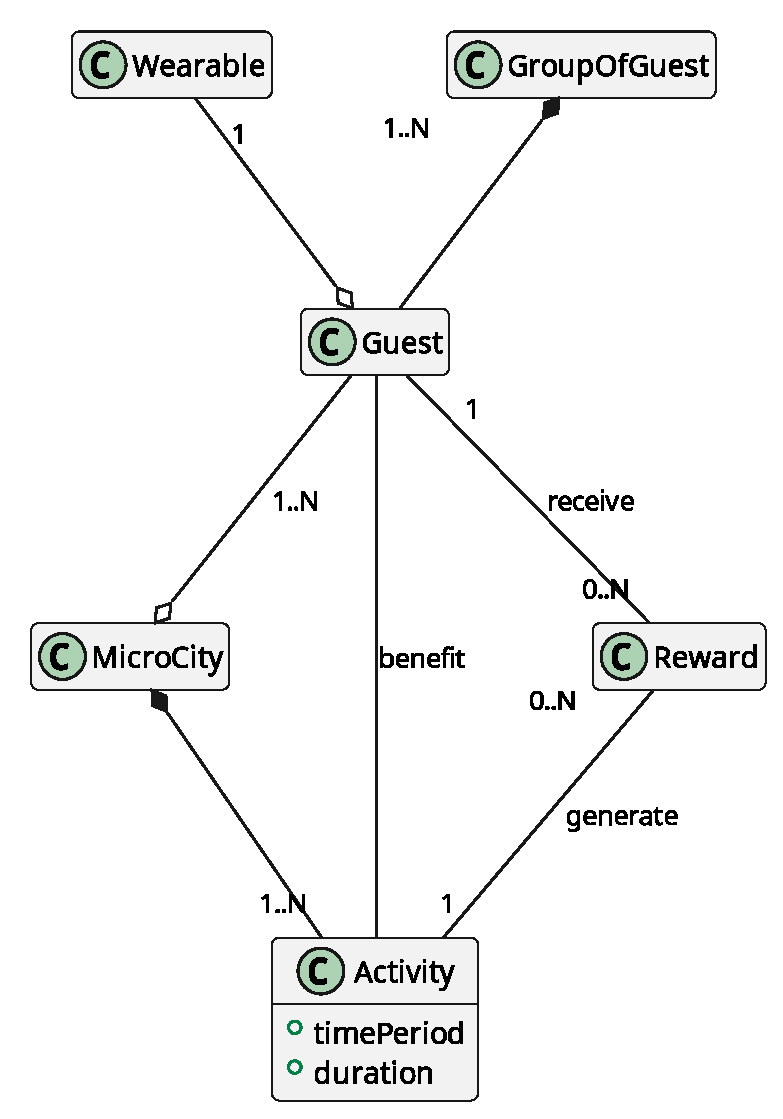
\includegraphics[width=0.55\textwidth]{./img/domain_overview-0}
	\caption{Class diagram of the \textit{Micro City}'s domain model.}
	\label{fig:domain-overview}
\end{figure}

\newpage

The figure \ref{fig:micro-city} shows a diagram representing the organization of a \textit{Micro City}.
A \textit{Micro City} has a map and many workers.
Both activities and the \textit{Micro City} itself may require the payment of a fee, that is an amount of money needed in order to access them.
There are two types of activities: services, that are continuously available during the \textit{Micro City}'s lifetime, and events, that take place in a specific moment and have a limited duration.
Queues may form because of the waiting time needed before a guest can benefit from an activity.

\begin{figure}[H]
	\centering
	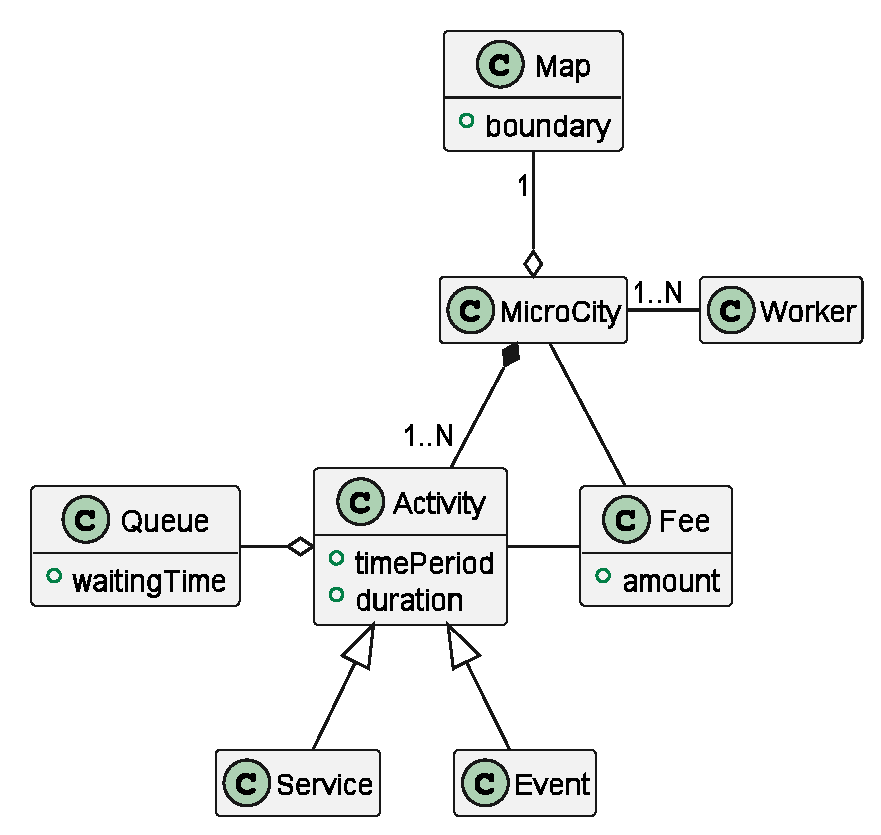
\includegraphics[width=0.7\textwidth]{img/micro_city-0.eps}
	\caption{Class diagram that models the organization of a \textit{Micro City}.}
	\label{fig:micro-city}
\end{figure}

\newpage

The figure \ref{fig:reward} shows the sequence diagram that explains how a guest can obtain a reward.

\begin{figure}[H]
	\centering
	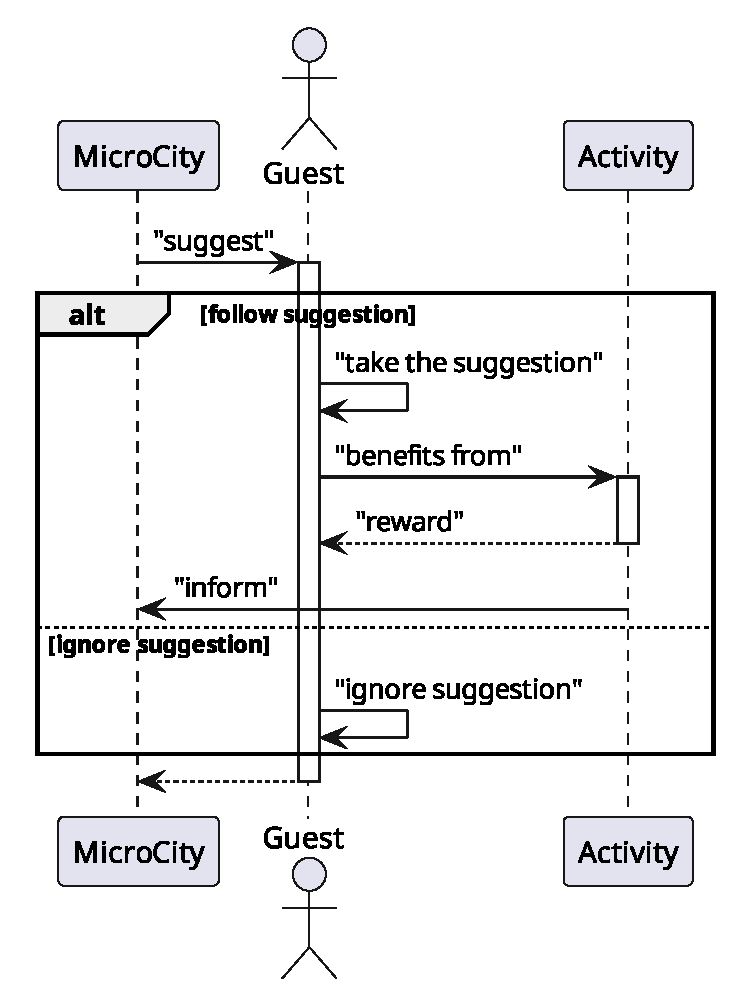
\includegraphics[width=0.6\textwidth]{./img/reward-0}
	\caption{Sequence diagram that shows how to obtain a reward.}
	\label{fig:reward}
\end{figure}

\newpage
\section{Application Scenarios}

This section describes some application scenarios for the \textit{Micro City}.
Some examples could be:

\begin{itemize}
	\item \textbf{Shopping Center} - In this context, the guests are the clients and their common objective is to benefit from services buying products sold by commercial activities.
	      The activities are shops and restaurants;
	      they may supply rewards in terms of discounts and cashbacks.
	\item \textbf{City Center} - In this context, the guests are the citizens and they move around a delimited area of the city center in search of events and shops.
	      In this case, the possible rewards might be discounts and cashbacks.
	\item \textbf{Amusement Park} - In this context, the guests are the visitors and they are interested in attractions, restaurants and shows.
	      In this case, the possible rewards may concern discounts and/or accumulable points, exploitable in commercial activities, or the reduction of the waiting time before entering an attraction.
	\item \textbf{Sports Center} - In this context, the guests are the athletes and their objective is to use fields, courts and pitches and participate in tournaments.
	      In this case, the possible rewards may be the reduction of waiting time before using a sports field.
\end{itemize}

\begin{table}[H]
	\centering
	\begin{tabular}{|l|l|l|p{.3\textwidth}|}
		\hline
		\textbf{Micro City} & \textbf{Guests} & \textbf{Activities} & \textbf{Rewards} \\
		\hline
		\case{Shopping Center}{Clients}{Shops}{Discounts/Cashbacks}
		\case{City Center}{Citizens}{Shops \& Events}{Discounts/Cashbacks}
		\case{Amusement Park}{Visitors}{Attractions \& Shows \& Shops}{Discounts/Waiting Time Reduction}
		\case{Fair}{Visitors}{Stands \& Shows}{Accumulable Points/ Waiting Time Reduction}
		\case{Sports Center}{Athletes}{Fields \& Tournaments}{Waiting Time Reduction}
	\end{tabular}
	\caption{Some examples of application cases.}
	\label{tab:examples}
\end{table}

\chapter{Case Study}\label{chap:case-study}
\section*{Introduction}\label{sec:introduction}
\addcontentsline{toc}{section}{Introduction}

This document has the purpose of mapping the \textit{Micro City}'s concepts into the amusement park's case study.
This allows to reach a common starting point for different future works.
Specifically, amusement parks will be analyzed defining a ubiquitous language of their domain.
This language will be useful to give a formal definition of the domain's elements.
Moreover, it will explain logic and semantic relationships among the elements of the domain.


\section{The Case Study}\label{sec:case}

As mentioned in the introduction, the case study of the \textit{Micro City} analyzed in this document is the one of amusement parks.
Amusement parks are considered to be a large business all around the world and attract people of every age and culture.
They satisfy the \textit{Micro City}'s spatial and temporal characteristics as most of them develop in a bounded spatial area and are open daily for a limited amount of hours.
Usually, they are not as wide as a city and grant access to visitors in the daylight hours.

Inside, they offer a large set of attractions that may vary depending on the type of amusement park.
For instance, they may be roller-coasters, carousels, water slides and many others.
Attractions correspond to \textit{services} in the current case study, as they offer experiences to \textit{guests}.
On the other hand, shows correspond to \textit{events}, as they take place at a specific time.
Usually, attractions are static, that is, they do not move.
Moreover, they satisfy a certain amount of guests within a limited duration: this time span is identified by the attraction's frequency, that is the rate at which the attraction starts a ride.
In most of the cases, attractions have one or many workers that decide when a ride can start depending on a set of environmental factors, different for every type of attraction.
The number of guests that are satisfied in a ride corresponds to the number of people that fit in the attraction.

Guests are embodied by visitors.
They are highly interested in the activities offered by the amusement park.
In fact, they attend the parks mainly for the attractions inside them.
They may attend the parks as single individuals (for instance, buying a personal ticket) or in groups.
It can be assumed that they own a personal wearable device used to receive information about attractions.
Also, it can be assumed that a group of guests uses a single wearable device for the same purpose.
An amusement park also presents internal operators, distinguished from guests, that do not benefit from attractions;
instead, they manage the attractions and help visitors.

An amusement park may have its personal business model and could require to pay a fee just to get inside the park itself.
Attractions inside the park can be free or could need a form of payment from visitors because they offer additional services or products, such as restaurants.

In this scenario, it could be useful to recommend the most suitable attraction to visitors depending on their physical location, tracked by their personal wearable device, or on their interests.
The recommendations may concern the nearest attraction that suits the visitor's preferences or an attraction with a short queue (compared to the average queue of the attraction, or compared to the queues of other attractions).
This mechanism could be referred as \textbf{situated recommendation}.
By accepting situated recommendations, visitors may receive a reward provided by the amusement park.
For instance, the most straightforward reward is the reduction of the waiting time in order to benefit from an attraction.

\section{Ubiquitous Language}
\label{sec:ubiquitous-language-cs}

The following table shows the ubiquitous language of the analyzed case study.

\begin{longtable}{|l|l|p{.4\textwidth}|}
	\hline
	\textbf{Term} & \textbf{Micro City's Term} & \textbf{Definition} \\
	\hline
	\ult{Amusement Park}{Micro City}{A large outdoor area with fairground rides, shows, and other entertainments.}
	\ult{Visitor}{Guest}{A person attending the amusement park.}
	\ult{Group of Visitors}{Group of Guests}{A set of visitors attending the amusement park.}
	\ult{Attraction}{Service}{Type of activity offered to visitors. An attraction is continuously available during the amusement park's lifetime and allows visitors to benefit from it at any time. They can be rides, roller coasters, water slides, but also restaurants or shops.}
	\ult{Show}{Event}{Type of activity offered to visitors. A show takes place in a specific moment and is carried out only once; when it terminates, it won't be available anymore.}
	\ult{Satisfy}{Satisfy}{The action of an attraction or a show of providing visitors with an experience or a product.}
	\ult{Benefit From/Attend}{Benefit From/Attend}{The act of a visitor of exploiting an attraction or a show and being satisfied by it.}
	\ult{Time Period}{Time Period}{An attraction's operation time span. It is defined by a start and an end.}
	\ult{Duration}{Duration}{The time taken by an attraction or a show to satisfy one or more visitors.}
	\ult{Waiting Time}{Waiting Time}{Amount of time that visitors wait before benefiting from an attraction or a show.}
	\ult{Queue}{Queue}{Set of aligned visitors due to long waiting time.}
	\ult{Wearable}{Wearable}{Device owned by each visitor (or group of visitors) that allows them to interact with the amusement park.}
	\ult{Recommendation}{Recommendation}{A proposal to benefit from a specific attraction or show in exchange for a reward.}
	\ult{Recommend}{Recommend}{The action of sending a recommendation to the visitors.}
	\ult{Reward}{Reward}{The recompense received by the visitors that accept a recommendation.}
	\caption{Ubiquitous language of the amusement park's case study.}
	\label{tab:ul-cs}
\end{longtable}

\section{Scenarios}\label{sec:scenarios}

Amusement parks surely represent a popular form of entertainment for people of all ages and with different interests.
This is one of the reasons why, specially during holiday times, these parks attract a considerable amount of visitors and tend to be significantly crowded.
Although this is greatly profitable for the parks themselves, unfortunately it is not the ideal situation for the visitors as chances are that they will have to spend most of their time waiting in a queue.
This situation becomes even more unattractive for large groups of visitors, such as families with children, or under unpleasant weather conditions, such as rain or summer heat.
In order to improve the overall visitors' experience, the \textbf{situated recommendation system} could suggest the most suitable attractions for them.

In addiction, such system could be also convenient for amusement parks' managers.
In fact, visitors would be more attracted to the parks providing such facilities, meaning that the attendance of visitors would increase.
Also, it is important mentioning that not all attractions inside the parks are rides or roller coasters.
In fact, parks can also contain restaurants or shops.
A situated recommendation regarding these kinds of attraction may involve marketing strategies that would make visitors willing to go there.
Given all the advantages that a service like that could provide to the visitors, managers could also decide to supply it as an additional ``premium" service.
\section{Requirements}\label{sec:requirements}

The \textbf{situated recommendation system} must satisfy the following business requirements in order to be appealing to amusement parks:
\begin{enumerate}
    \item The ability to make recommendations based on certain criteria.
    Thus, it should be able to access information about the park in order to elaborate an as desirable as possible recommendation for the visitors.
    It is not important to focus on the way the recommendation is generated.
    Instead, it should be able to define different strategies and use the most suitable one.
    For instance, some strategies may be based on the length of queues or visitors' interests.
    \item The ability to keep track of the state of every attraction inside the park.
    In such a way, it would be possible to provide not only static recommendations (for instance based on the visitors' preferences) but also dynamic ones.
    The latter may be based on attractions' information such as their current queue, their duration, their capacity, etc.
    \item The ability to keep track of the state of every visitor (or group of visitors) inside the park.
    In this way, it would be possible to provide them with recommendations based on their interests and their physical location.
    Thus, visitors would be more satisfied as they would benefit from attractions they surely enjoy.
    Moreover, it could be possible to suggest attractions near to them in order to minimize the walking time.
    \item The possibility to memorize the information collected during the amusement park's lifetime.
    This allows the parks' managers to analyze trends and visitors' preferences in order to make improvements to their attractions or promote others.
    Moreover, this could help them develop new recommendation strategies that might be more effective.
\end{enumerate}

\chapter{Mirabilandia Case Study}\label{chap:mira-case-study}
\section*{Introduction}
\addcontentsline{toc}{section}{Introduction}
\label{sec:introduction}

The objective of this chapter is to describe the current Mirabilandia amusement park's situation in terms of technologies used in its business and to offer an overview of other parks that already use some suitable technologies for the Micro City context.
Finally, it will be illustrated a potential architecture for a future Mirabilandia improved with all of the characteristics of a Micro City.

In table~\ref{tab:terms}, is listed the terminology of the Micro City context -- specifically for the amusement parks, extracted from the case study ubiquitous language -- which will be used in the document from now on.

\begin{longtable}{|l|p{.4\textwidth}|}
	\hline
	\textbf{Term} & \textbf{Definition} \\
	\hline
	\ul{Visitor}{A person attending the amusement park.}
	\ul{Group of Visitors}{A set of visitors attending the amusement park.}
	\ul{Attraction}{Type of activity offered to visitors. An attraction is continuously available during the amusement park's lifetime and allows visitors to benefit from it at any time. They can be rides, roller coasters, water slides, but also restaurants or shops.}
	\ul{Show}{Type of activity offered to visitors. A show takes place in a specific moment and is carried out only once; when it terminates, it won't be available anymore.}
	\ul{Wearable}{Device owned by each visitor (or group of visitors) that allows them to interact with the amusement park.}
	\ul{Recommendation}{A proposal to benefit from a specific attraction or show in exchange for a reward.}
	\ul{Recommend}{The action of sending a recommendation to the visitors.}
	\ul{Reward}{The recompense received by the visitors that accept a recommendation.}
	\caption{Terms that will be used in the following chapters.}
	\label{tab:terms}
\end{longtable}
\section{Mirabilandia today}\label{sec:mirabilandia-today}
The amusement park to date offers limited technological support to visitors, as a result, all activities are carried out in a "traditional" manner:
for instance, there is no technological support for queue management, they only provide the
``Flash Pass''\footnote{\url{https://www.mirabilandia.it/en/organizza-la-tua-visita/attivita/flash-pass}} (a paper card or bracelet that gives you
priority access to the attractions by a reserved entrance) that has no virtual queueing system integration.
In addition, there is no system to improve the visitor experience based on either the visitor's preferences or external factors that may affect the
quality of their visit.

There are some "totems" placed around the park that give information about the attractions and the current waiting time.

However, we have no information on how the waiting time is calculated and, based on empiric considerations, it turns out to be approximate and not very indicative of reality.
In figure~\ref{fig:mira-totem} there is an example of a totem placed in the park.

\begin{figure}[H]
	\centering
	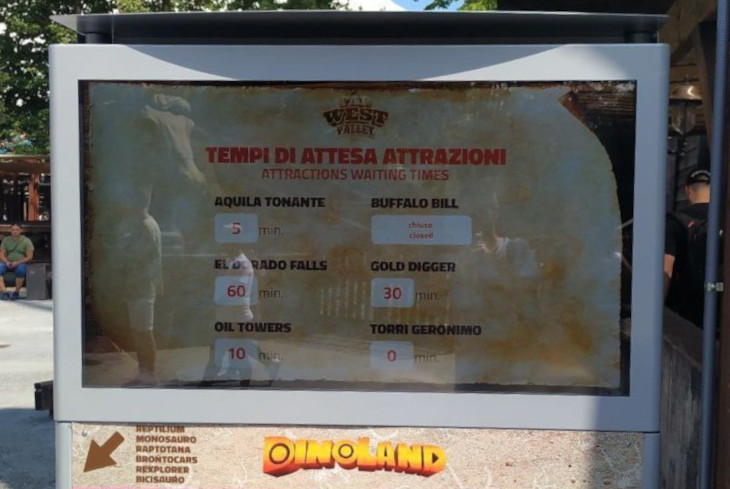
\includegraphics[width=0.8\textwidth]{img/mira-totem.jpg}
	\caption{A totem showing the average waiting time for each attraction in the Mirabilandia park.}
	\label{fig:mira-totem}
\end{figure}

Mirabilandia provides a very simple app\footnote{\url{https://www.mirabilandia.it/en/prima-del-tuo-arrivo/la-nostra-app}} for smartphones that, however, doesn't have the characteristics needed for an actual Micro City experience.
In fact, allows the \textit{visitors} to:
\begin{itemize}
	\item buy tickets
	\item consult an interactive map
	\item visualize pre-defined and static itineraries
	\item consult shows' beginning time
	\item select a pre-defined and static plan by attraction's category: ``extreme'', ``for families'', ``wet'', ``for families'' and ``for children'' (Figure\ref{fig:miraApp})
\end{itemize}

Lastly, Mirabilandia offers a very simple virtual queueing service Qoda\footnote{\url{https://get.qoda.app/}} for three refreshment points and stores\footnote{\url{https://www.mirabilandia.it/mir-blog-export/qoda-la-tua-fila-virtuale}}.
It works by scanning a QR code one can find at the point of interest and it will immediately tell the waiting number on the person's mobile phone, as well as the estimated time for their turn.

\begin{figure}[H]
	\centering
	\begin{subfigure}[b]{0.35\textwidth}
		\centering
		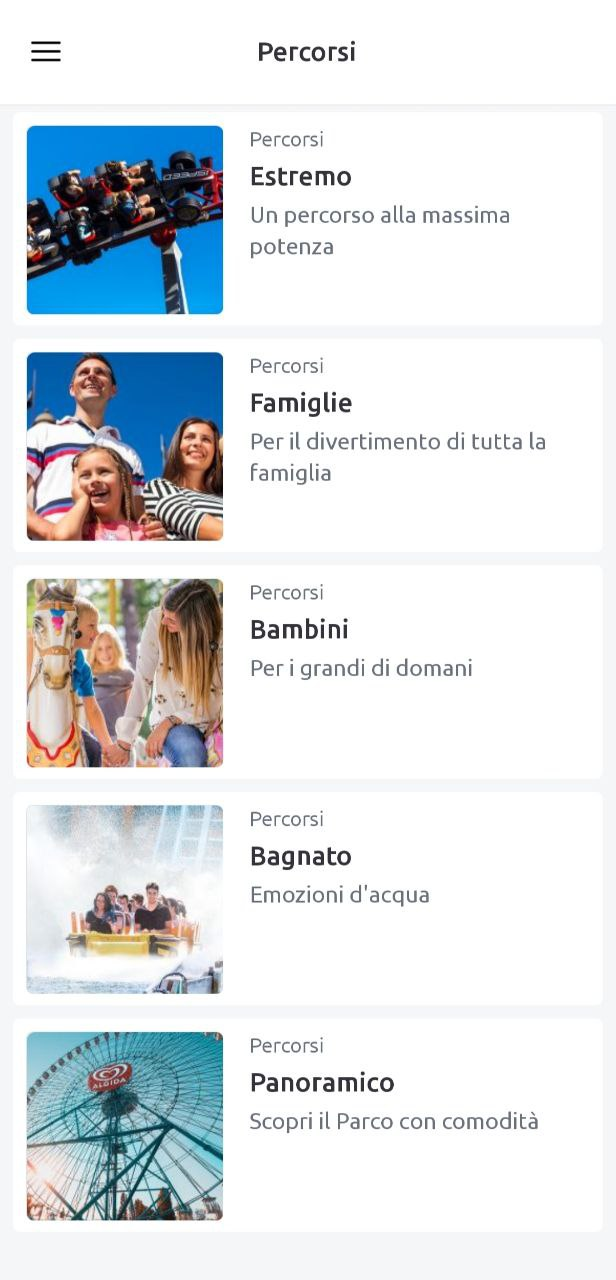
\includegraphics[width=\textwidth]{img/miraPlan}
	\end{subfigure}
	\begin{subfigure}[b]{0.35\textwidth}
		\centering
		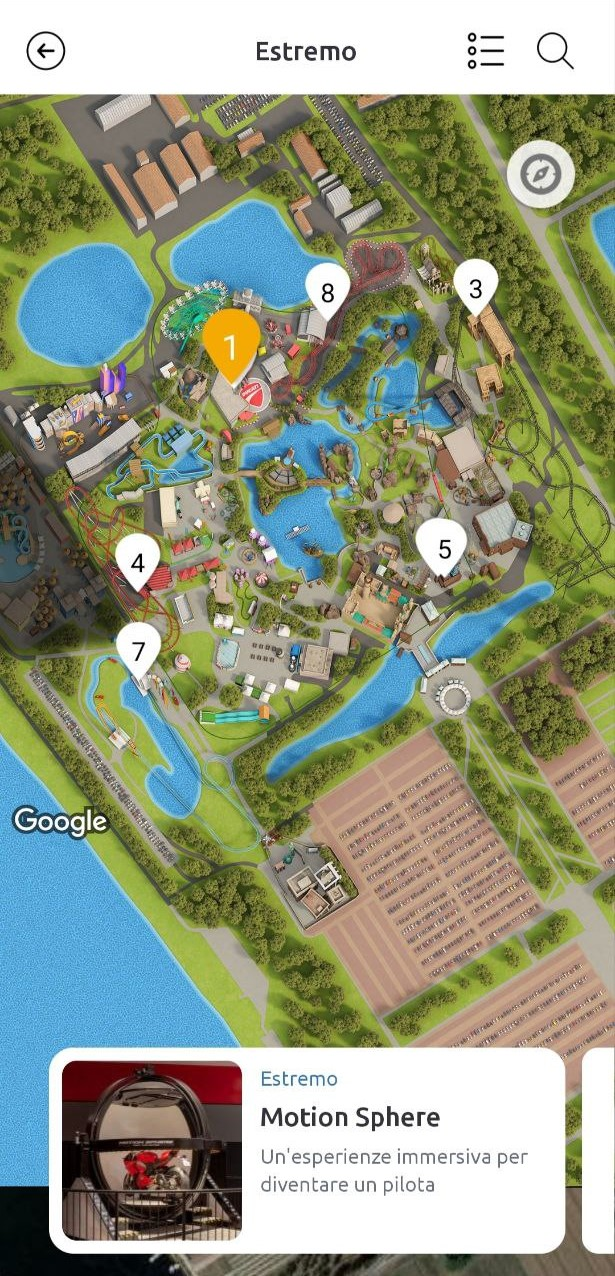
\includegraphics[width=\textwidth]{img/miraextr}
	\end{subfigure}
	\caption{Mirabilandia App's planning a visit screenshots}
	\label{fig:miraApp}
\end{figure}

% Queues at the various attractions are still conducted traditionally, without any technological support.
% At present, Mirabilandia amusement park does not have a queue management system or a recommendation system for its guests.
% The amusement park only provides totems that indicate an average wait time for each attraction.
% However, the stated time turns out to be very often approximate and not very indicative of reality.
% In recent years, the ``flash pass'', a facility that allows guest to skip the line, has been introduced.
% Again, such a system has no technological support: guests must go to the ride in advance and indicate the time they intend to participate.

% Mirabilandia does not currently provide any recommendation system: all activities within the park are independent and do not actively collaborate
% with it to incentivize guests to interact with these activities.

\section{Currently available services and technologies for smart amusement parks}\label{sec:state-of-the-art-analysis}
This section will discuss the state of the art of technologies already used in amusement parks around the world.
It will also focus on those used, or that have been used in the past, in the Mirabilandia park in Italy.
The main purpose is to understand what would be the best ``smart'' and innovative technological options to use in Mirabilandia nowadays considering the Micro City context.
As seen in the documents ``Micro City - Domain Analysis'' and ``Micro City - Case Study Analysis'', an Amusement Park as a Micro City has the following necessities:
\begin{itemize}
	\item Queue management: the park may want to offer its visitors the possibility of reducing the waiting time to access an attraction, event or a food service
	\item Personalization of the experience: recommendation systems may be used by the park to suggest attractions, restaurants, events, etc.
	      based on the visitors' interests
	\item Proximity/localization suggestions: visitors may receive on their wearable device some notifications concerning marketing, offers or the queue with fewer wait-time based on their position within the park
\end{itemize}

There are many solutions adopted by some amusement parks to support the previous points.
For instance, the avoiding long lines problem is faced with virtual queueing\footnote{\url{https://en.wikipedia.org/wiki/Virtual_queue}} systems
and for recommendation and proximity marketing\footnote{\url{https://en.wikipedia.org/wiki/Proximity_marketing}} there are many different solutions.

The following sections are intended to provide an overview of companies' products and technologies already used in amusement parks around the world,
as well as Mirabilandia's current offer in terms of smart services.

\subsection{Accesso Technology Group}\label{subsec:accesso-technology-group}
Accesso Technology Group\footnote{\url{https://www.accesso.com/}} (formerly Lo-Q) is an English company that provides different solutions
mostly to amusement parks like the ``Six Flags'' corporation in the US and ``LEGOLAND Windsor Resort'' in the UK but also to airports,
ski facilities, events and places that need social distancing management and so on.
Their two main solutions of interest for a Micro City context are a virtual queueing system and the personalization of
the \textit{visitors}' experience by sending them tailored contents, offers and recommendations.
Furthermore, along with their virtual queueing products they integrate a location-based messaging system.

\subsubsection{Lo-Queue Virtual Queueing Products}
Their patented~\cite{q-management-system-patent} \cite{q-system-patent}
virtual queueing technology allows a virtual queue to dynamically adjusts to many different unpredictable real-time variables such
as guest flow, bad weather, ride down time, etc.
automatically revising wait times and communicating real-time updates to \textit{visitors}.
The mechanism, simply lets the visitors choose a ride and, when their turn comes, are notified to head to the attraction.

Their two current products for virtual queueing are \textit{Qsmart} and \textit{Prism}\footnote{\url{https://www.accesso.com/solutions/virtual-queuing/prism}}.
The former allows people to access the virtual queueing services directly from their smartphones, whereas the latter is a ``smartwatch-like''
wearable.

In 2009, Mirabilandia used to sell to its \textit{visitors} the Accesso's \textit{Qbot} device -- a previous version of Prism -- named ``V-Pass''\cite{v-pass-mira}, but is no
longer available to this days.

\subsubsection*{Prism}
Prism is a standalone device, with no need for kiosks or charging stations to support its use.
Moreover, it is waterproof, hypoallergenic and durable~\cite{prism-desc}.
As can be observed in Figure~\ref{fig:prism}, Prism provides the following functionalities:
\begin{itemize}
	\item Virtual queueing: \textit{visitors} can manage their reservation in line and monitor the line status
	\item Payments: \textit{visitors} can make payments via secure NFC technology
	\item Messaging: \textit{visitors} can receive push notifications for proximity-based marketing (i.e.\ trigger nearby events based on people location, Figure~\ref{fig:prism-icecream}), operational updates, or the status of pending virtual queue positions
	\item Photography: Prism allows automated tagging of ride and park photographs
	\item Access: \textit{visitors} can easily access park turnstiles, guest lockers, resort hotel rooms, etc.
	\item Intelligence: Prism collects real-time information about the users' behaviour during the visit for marketing and park operations purposes
\end{itemize}

\begin{figure}[H]
	\centering
	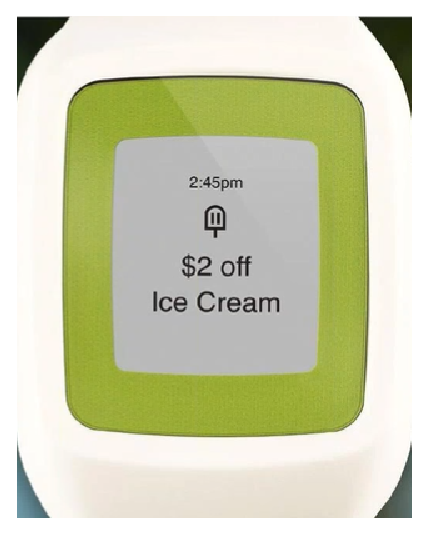
\includegraphics[width=0.3\textwidth]{img/prism-icecream}
	\caption{Example of a push notification based on the visitor proximity to an ice cream shop}
	\label{fig:prism-icecream}
\end{figure}

In addition to their patented virtual queueing technologies, Prism works on a \textbf{proprietary network} and uses three ways to communicate:
\begin{itemize}
	\item \textbf{Bluetooth Low Energy:} allows \textit{visitors} to receive real-time messages based on their location, and the park gains valuable insights about visitors' flow throughout the park
	\item \textbf{Near Field Communication (NFC):} used for access, payments, rentals, etc.
	\item \textbf{Long Range Sub-GHz Two-Way Radio:} allows \textit{visitors} to reserve and modify queueing reservations from where they are without having to use their smartphone
\end{itemize}

The wearable is made with waterproof materials and carries a vibrator motor for haptic feedback to interact with the user and send alerts.
Moreover, its battery supports over 200 days of usage.
Technical specifications~\cite{prism-manual} are listed in Tables~\ref{tab:ci-tec-spec},~\ref{tab:pr-tec-spec},~\ref{tab:c-tec-spec}.

\begin{table}[H]
	\centering
	\begin{subtable}[t]{0.85\textwidth}
		\centering
		\begin{tabular}{|l|l|}
			\hline
			LCD            & LCD Display, 3 bit colour, Resolution 176 x 176 \\ \hline
			Vibrator motor & 1,000 rpm                                       \\
			\hline
		\end{tabular}
		\caption{Controls and Indicators}
		\label{tab:ci-tec-spec}
	\end{subtable}
	\begin{subtable}[t]{0.85\textwidth}
		\centering
		\begin{tabular}{|l|l|}
			\hline
			Battery      & CR3032 Lithium Ion coin cell \\ \hline
			Average life & 200 days or 2,000 hours      \\
			\hline
		\end{tabular}
		\caption{Power Requirements}
		\label{tab:pr-tec-spec}
	\end{subtable}
	\begin{subtable}[t]{0.85\textwidth}
		\centering
		\begin{tabular}{|l|l|}
			\hline
			Long Range   & 868MHz \& 915MHz (SubGHz) transceiver \\ \hline
			Medium Range & 2.4GHz BLE transceiver                \\ \hline
			Short Range  & Secure 14443 RFID/NFC device          \\
			\hline
		\end{tabular}
		\caption{Communications}
		\label{tab:c-tec-spec}
	\end{subtable}
	\caption{Prism technical specifications}
	\label{tab:prism-tech-spec}
\end{table}

\subsubsection*{QSmart}
On the other hand, QSmart is a ready-to-use platform and utilizes the visitor's smartphone hardware, is cloud based
and operates via Wi-Fi.

In addition to the features already listed for Prism, Qsmart gives the possibility to easily make rides and
show ticket purchases -- with its mobile payments system which is
PCI\footnote{\url{https://en.wikipedia.org/wiki/Payment_Card_Industry_Data_Security_Standard}} compliant --,
allows choosing among a different set of ride packages with different perks depending on the price, validating the
ride by a ride attendant -- who scans a QR code on the visitor's smartphone -- and it can be integrated with other Accesso's products like, for instance, an online ticketing system.


\begin{figure}[H]
	\centering
	\begin{subfigure}[b]{0.85\textwidth}
		\centering
		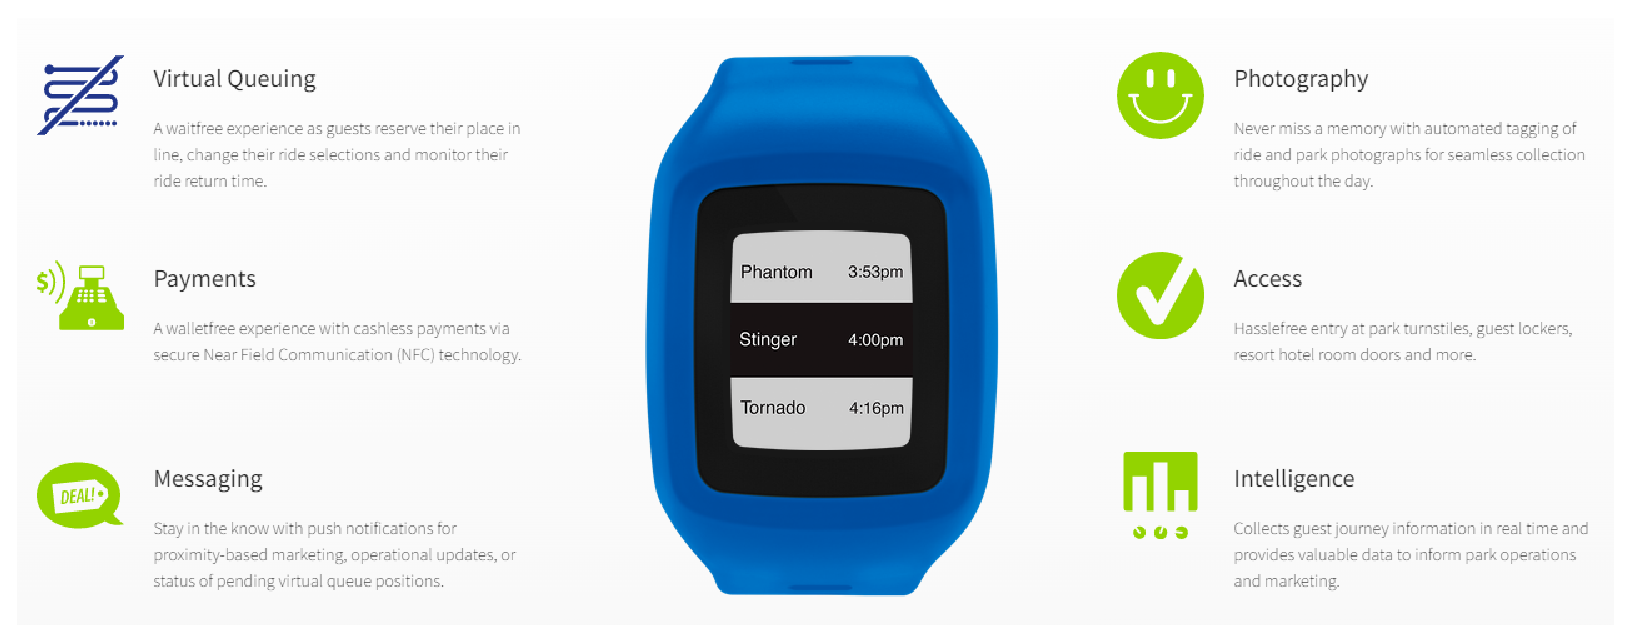
\includegraphics[width=\textwidth]{img/prism}
		\caption{Prism main functionalities}
		\label{fig:prism}
	\end{subfigure}
	\hfill
	\begin{subfigure}[b]{0.85\textwidth}
		\centering
		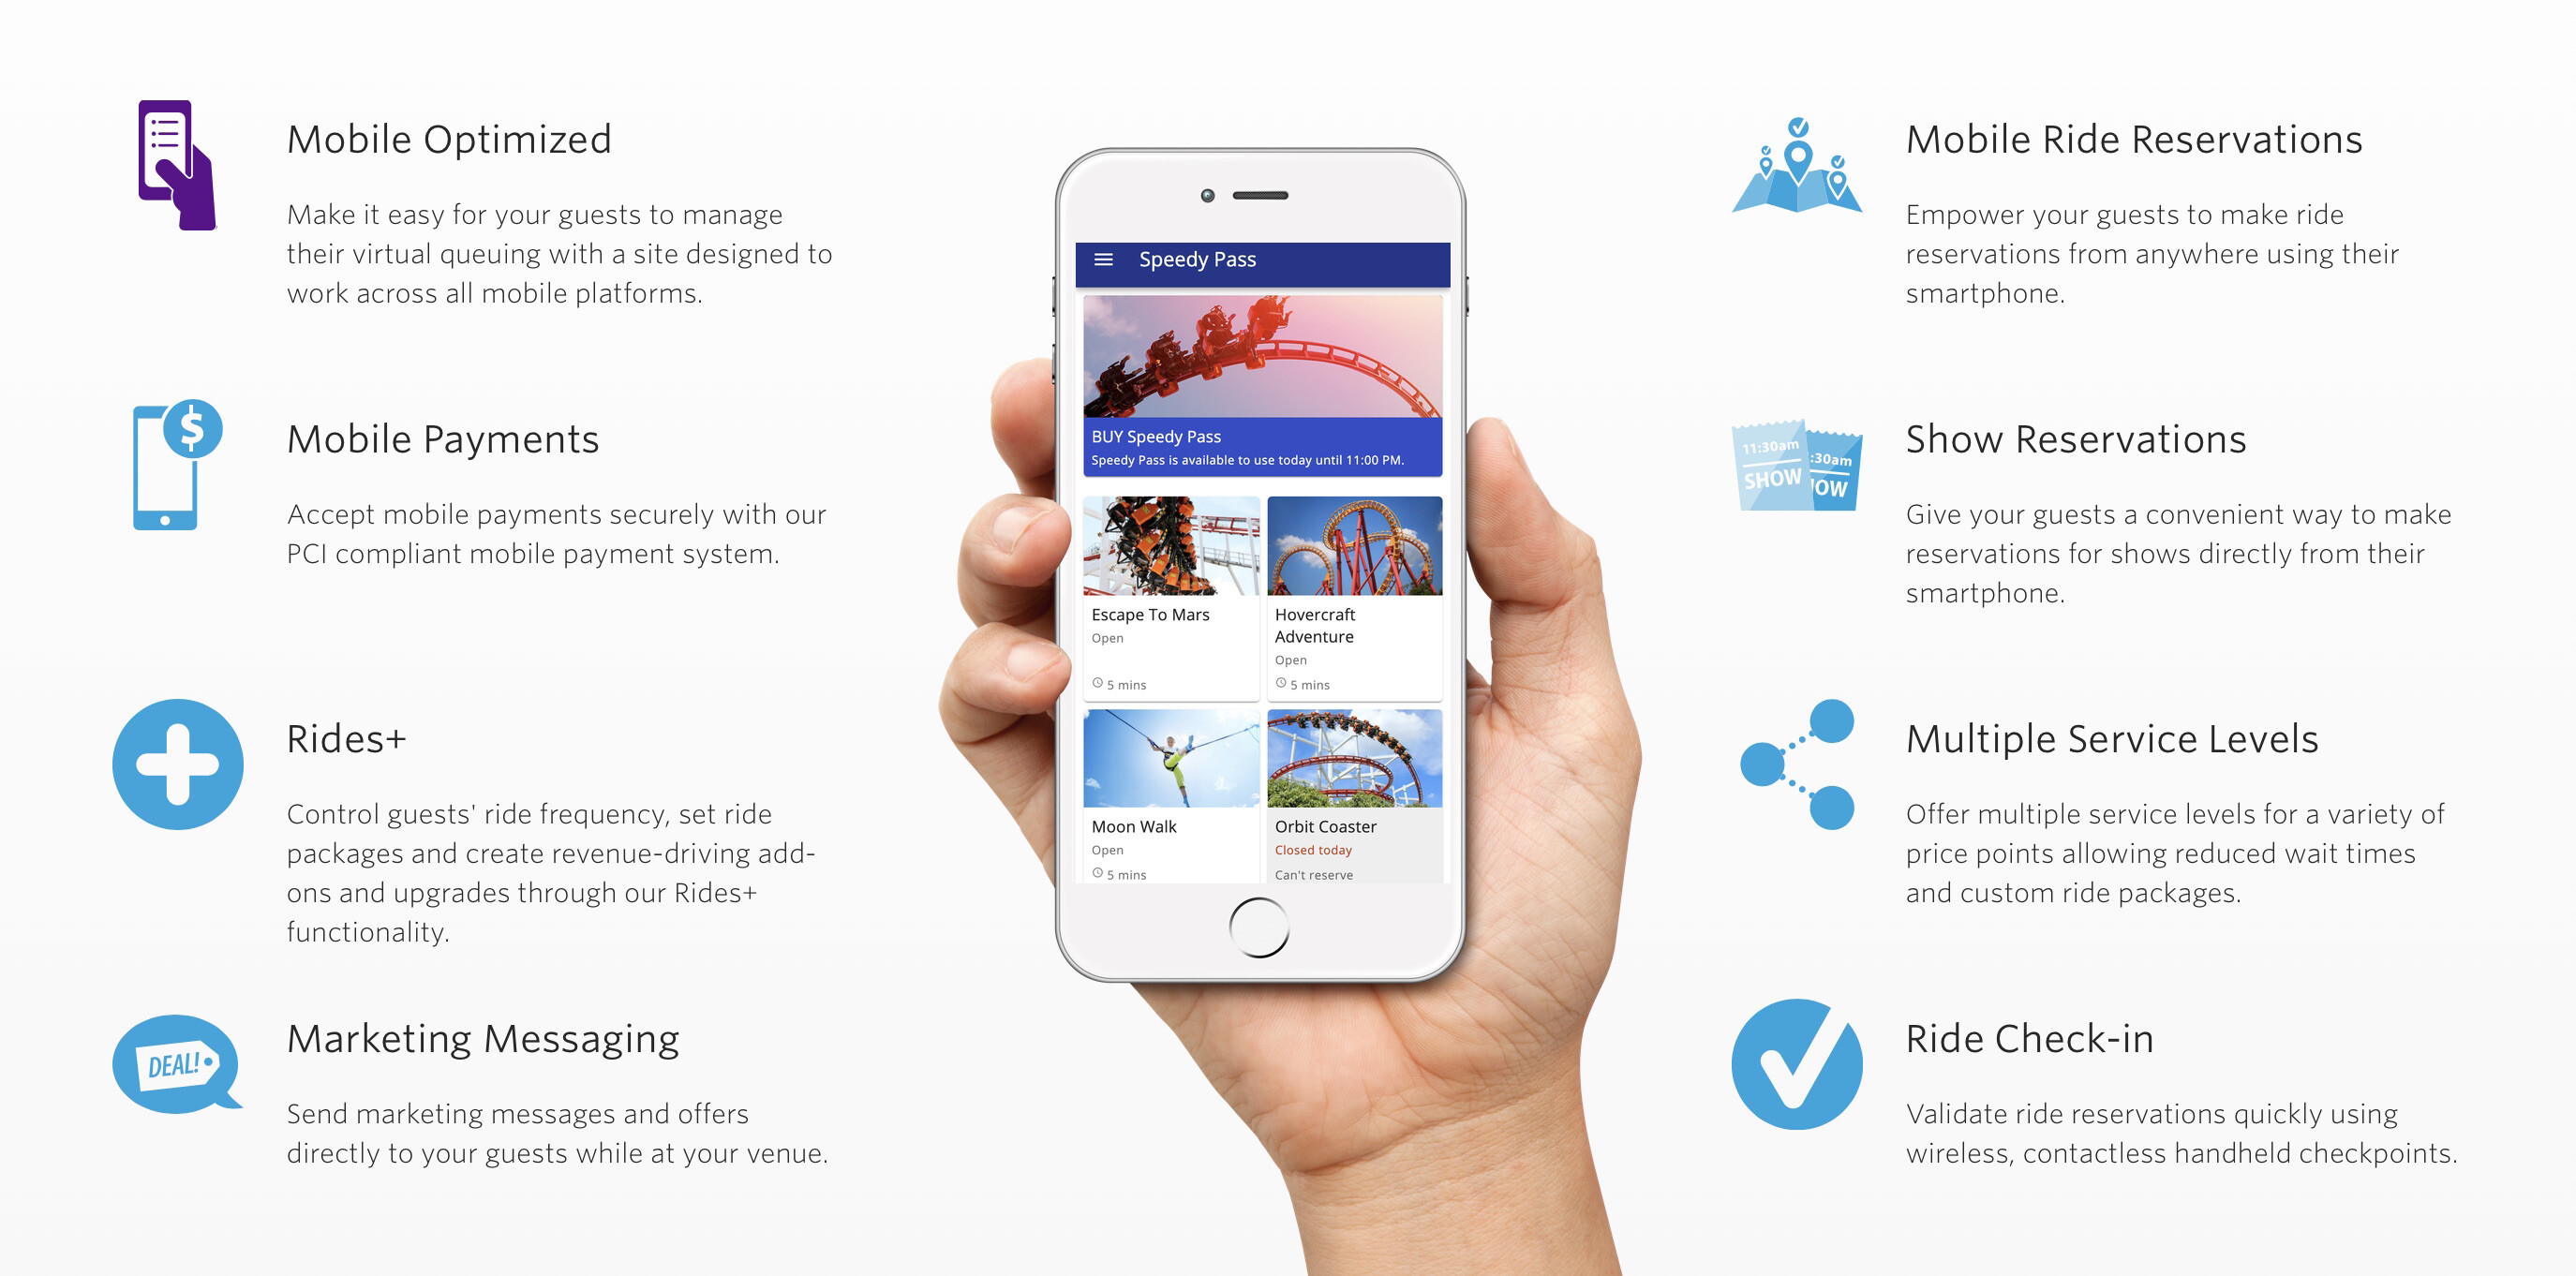
\includegraphics[width=\textwidth]{img/qsmart}
		\caption{Qsmart main functionalities}
		\label{fig:qsmart}
	\end{subfigure}
	\caption{Accesso's products for virtual queueing\protect\footnotemark}
	\label{fig:prismart}
\end{figure}
\footnotetext{\url{https://www.accesso.com/solutions/virtual-queuing}}

Both Prism and QSmart interact with the Virtual Queue Management System, where customers can consult
analytics and performance data as well as centralized data on park attendance.
It is also possible to check ride usage, \textit{visitors} activity, ride downtime and transactional data per user and how long they waited for each ride.
Finally, it is possible to control in real-time the virtual queueing solution.

\subsubsection{The Experience Engine (TE2) Recommendation system}
The Experience Engine\footnote{\url{https://www.accesso.com/solutions/guest-experience}} is a platform-as-a-service (PaaS) technology
which allows the park to connect with \textit{visitors} in real-time and provides them with relevant offers, messages and recommendations.
It is integrated with Accesso's Virtual Queueing Products and could work as a location-based targeted system~\cite{accesso-location-based-exp} helping alleviate
long lines by driving traffic to other less utilized outlets, or by incentivizing guests to dine before or after the rush
hours with special offers.
The platform communicates with Bluetooth Beacons\footnote{\url{https://en.wikipedia.org/wiki/Bluetooth_low_energy_beacon}} and,
whenever a visitor's device receives a beacon signal, the device notifies the TE2 platform of the proximity to a beacon.
TE2 then determines the visitor's real interest in a scheduled experience.
If so, the visitor will receive a notification.
Thanks to this platform, Accesso's clients can create custom itineraries for every park's visitor.
In Figure~\ref{fig:te2ex} is synthesized the TE2 functioning.

\begin{figure}[H]
	\centering
	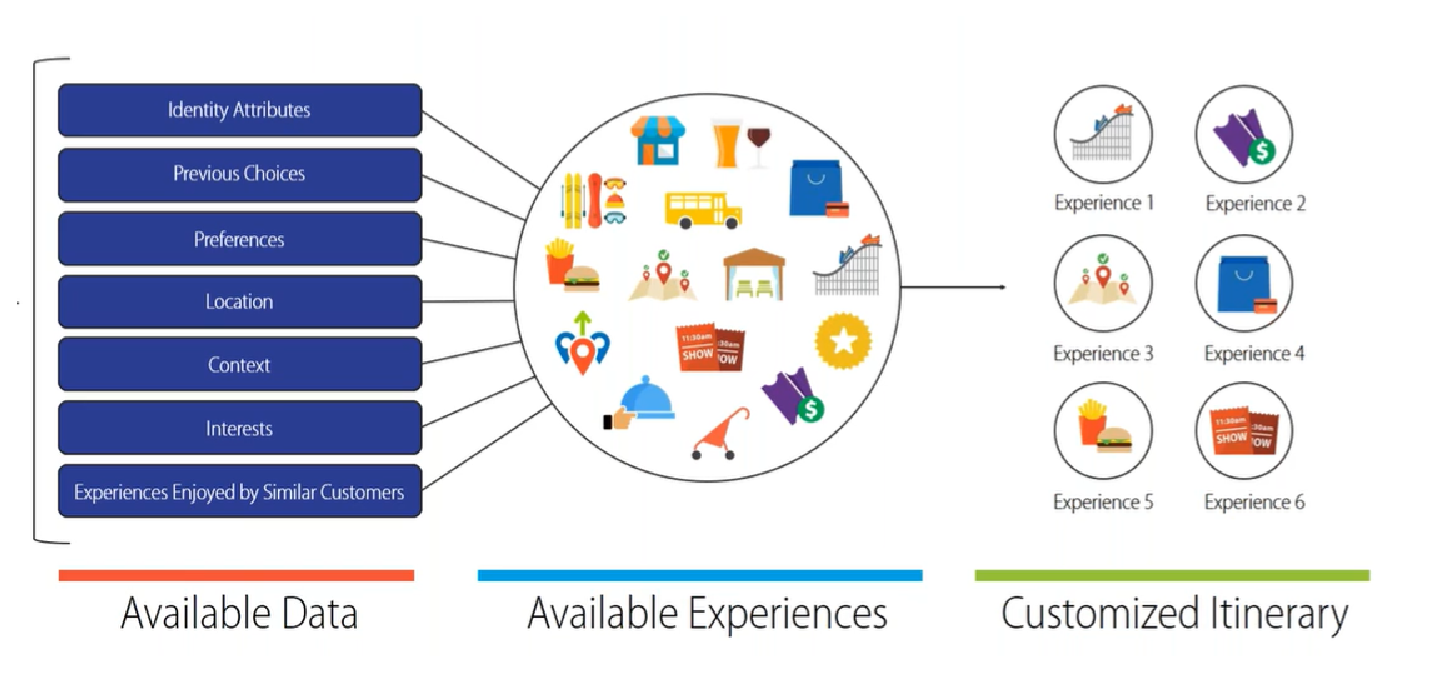
\includegraphics[width=0.9\textwidth]{img/te2ex}
	\caption{TE2 functioning}
	\label{fig:te2ex}
\end{figure}

\subsection{Disney Parks, Experiences and Products}\label{subsec:disney-parks-experiences-and-products}
Disney Parks, Experiences and Products, Inc., is one of The Walt Disney Company's business.
In its parks ``Walt Disney World'', Florida and ``Disneyland Resort'', California offers their \textit{visitors} solutions
for virtual queuing and a recommendation.
In fact, guests can use the ``My Disney Experience'' app and enjoy the ``Disney Genie'', ``Disney Genie+'' and ``Lighting Lane''\footnote{\url{https://www.disneyworld.eu/genie/information/}} services.
The former is free of charge whether ``Genie+'' and ``Lighting Lane'' have additional costs.
The perks in Figure\ref{fig:dgenie} are the following:

\begin{itemize}
	\item Tailored recommendations: \textit{visitors} can receive attraction and dining recommendations based on what is the preferred visiting plan they previously told
	      to the service
	\item Virtual assistant: provides a virtual assistant to ask questions about the park
	\item Time-based suggestions: it displays a good time to go to a suggested experience and an idea of the forecasted wait for attractions, entertainment and dining
	\item Booking \textit{activities}: order food, make dining reservations, check into a restaurant, request to join an available virtual queue or book arrival times in a reserved entrance for
	      some activities.
\end{itemize}

\begin{figure}[H]
	\centering
	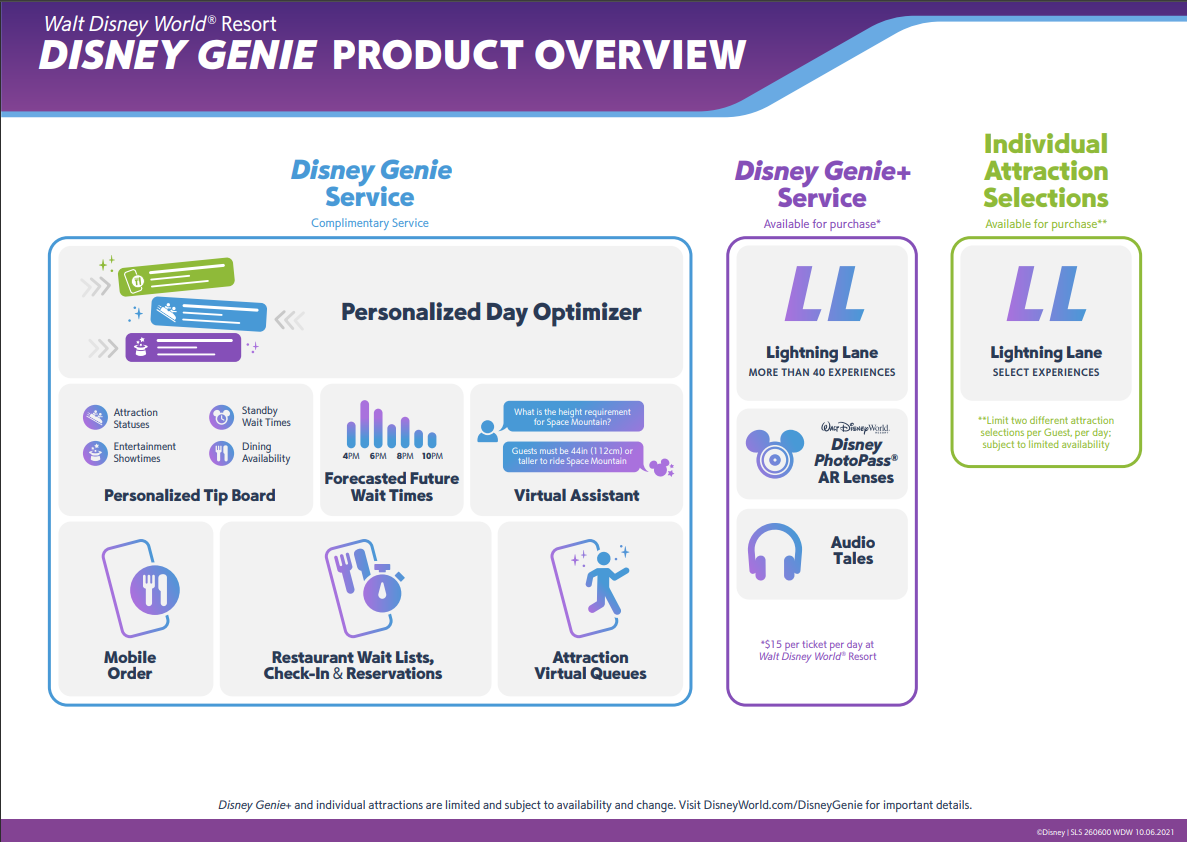
\includegraphics[width=0.8\textwidth]{img/dgenie}
	\caption{Disney Genie services}
	\label{fig:dgenie}
\end{figure}


\chapter{Mirabilandia as a Micro City}\label{chap:mira-micro-city}
\section{Overview}\label{sec:overview}
The objective of this chapter is to provide our solution to transform Mirabilandia into a Micro City analyzing the architectural requirements, the
technologies and providing concrete solutions.

We will illustrate an architecture with all the components needed to satisfy the characteristics of an amusement park as a Micro City: offer a
tailored and dynamic experience based on visitors' preferences and a situated recommendation system (Section~\ref{sec:requirements}) with a rewards
system.

The goal of the architecture section is to define a way to keep track of visitors' position within the park, provide a recommendation and reward
system, a way to smartly manage queues and visitors' information as well as provide a customizable plan of a day in the park.

As per the recommendation and reward systems, is important to point out their tightly coupled relationship since every suggested action provides some
kind of recompense. In ~\ref{tab:actions-rewards} are listed some examples of this relationship.

\begin{longtable}{|l|l|}
	\hline
	\textbf{Action}                         & \textbf{Reward}                              \\
	\hline
	This show is starting in 5 minutes      & You can get a reserved seat in the front row \\
	\hline
	If you go to this roller coaster        & You can get a reduced queueing waiting time  \\
	\hline
	If you go to this shop                  & You can get a discount on t-shirts           \\
	\hline
	Throw the plastic bottle in a smart bin & You can get a coin for the arcade            \\
	\hline
	\caption{Possible actions within Mirabilandia as a Micro City and their respective reward.}
	\label{tab:actions-rewards}
\end{longtable}

After the architecture description, we will explore suitable technologies for our case study, showing their possible use applied to Mirabilandia.

Finally, we will discuss possible deployment techniques in the park environment.

\section{Overall architecture}\label{sec:mira-microcity}
Following the analysis of the ``as-is'' system and the goals set to adapt the Micro-City concept to Mirabilandia,
figure~\ref{fig:architecture-overview} shows the component diagram that models the entities involved and the main relationships between them.

The main components of the system are the following:

\begin{itemize}
	\item \textit{Map Manager:} is responsible for tracking the visitors within the park and providing information about their current position
	\item \textit{Virtual Queueing System:} is responsible for managing the virtual queue for each attraction
	\item \textit{Recommendation System:} is responsible for providing recommendations to the visitors based on different factors that will be further discussed in the next sections
	\item \textit{Planner:} is responsible for planning the itinerary of the visitors based on their preferences and the crowding of rides
	\item \textit{Visitor Manager:} is responsible for the management of the users' information, preferences and tickets selling
\end{itemize}

\begin{figure}[H]
	\centering
	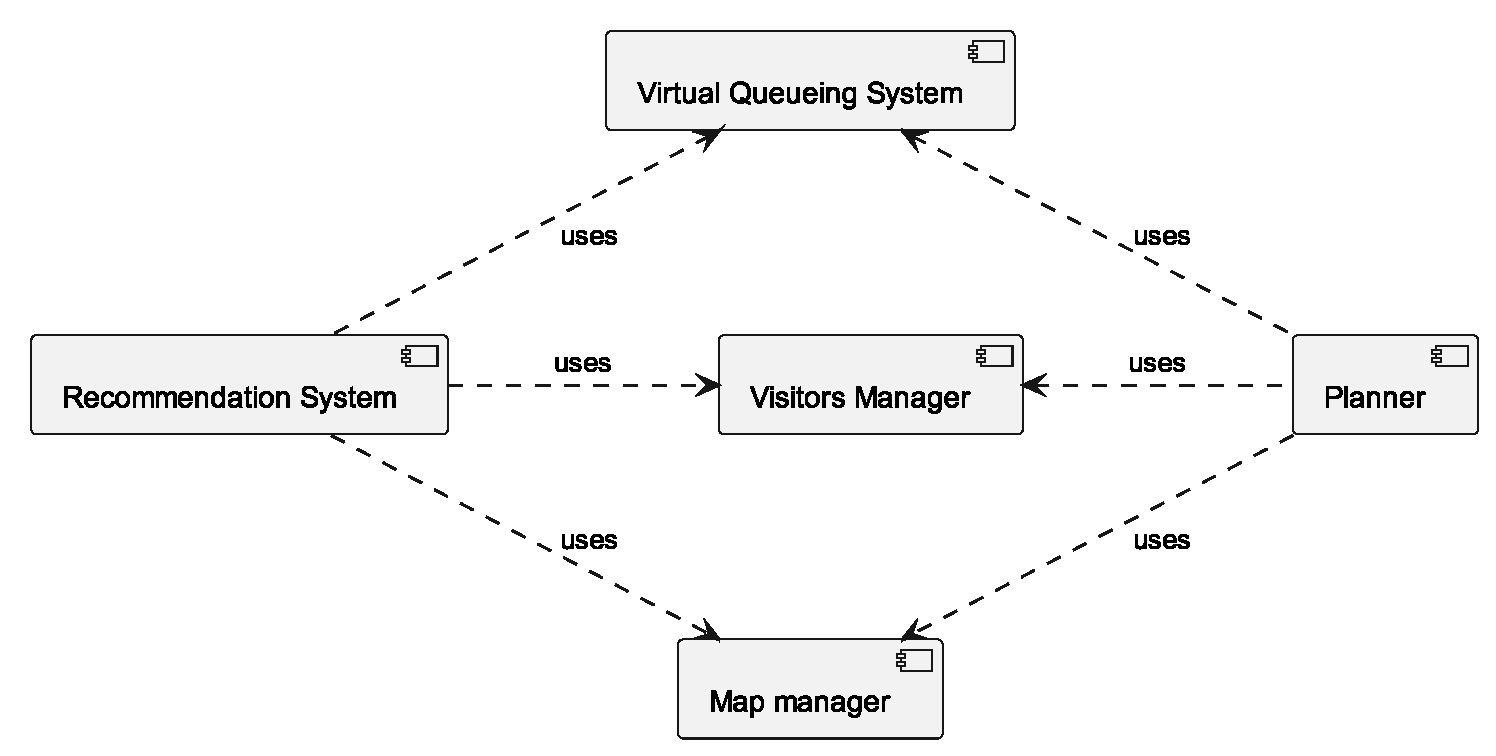
\includegraphics[width=0.9\textwidth]{img/architecture-overview.eps}
	\caption{Overall architecture of the Mirabilandia Micro-City.
		The Component Diagram shows the rough architecture and the main dependencies between the elements.
	}
	\label{fig:architecture-overview}
\end{figure}

From the diagram emerge that \textit{Map Manager}, \textit{Virtual Queueing System} and the \textit{Visitors Manager} are the main components of the
system since they are the ones that provide information to the other components. The \textit{Map Manager} provides information about the current
position of the guests to the \textit{Recommendation System} which uses this information to provide recommendations to the guests. Moreover, gives
information also to the \textit{Planner} to avoid crowd situations and maintain a uniform distribution of guests in the park. The \textit{Virtual
	Queueing System} is used by the \textit{Planner} to plan the itinerary of the guests and adapt it to reduce the waiting time and improve the quality
of the visit within the park and by the \textit{Recommendation System} to fetch information about the visitor's preferences and opportunistically
advise the attraction. The \textit{Visitor Manager} provides information to the \textit{Recommendation System} and the \textit{Planner} regarding
pre-defined users' preferences.

\section{Map Manager}

The location of visitors within the amusement park is critical for several reasons: it is used to make recommendations and to determine the best plan
for each visitor. So, a good tracking system is crucial for the correct working of the overall system.

The \textit{Map Manager} is composed of the following elements:
\begin{itemize}
	\item \textit{Device Information Ingestion:} receives from the visitors' devices information that can be used to estimate their current location. This component is the entry point of the \textit{Map Manger}.
	\item \textit{Location Inference:} is responsible for calculating the position of the visitors based on the information received from the
	      \textit{Device Information Ingestion} component. This component leverage \textit{Location Data} to calculate the position.
	      Finally, this component exposes an interface to provide the current position of the visitors to other components requiring information about visitors' positions within the park.
\end{itemize}

The figure~\ref{fig:map-manager} shows the component diagram that models the \textit{Map Manager} internal architecture.

\begin{figure}[H]
	\centering
	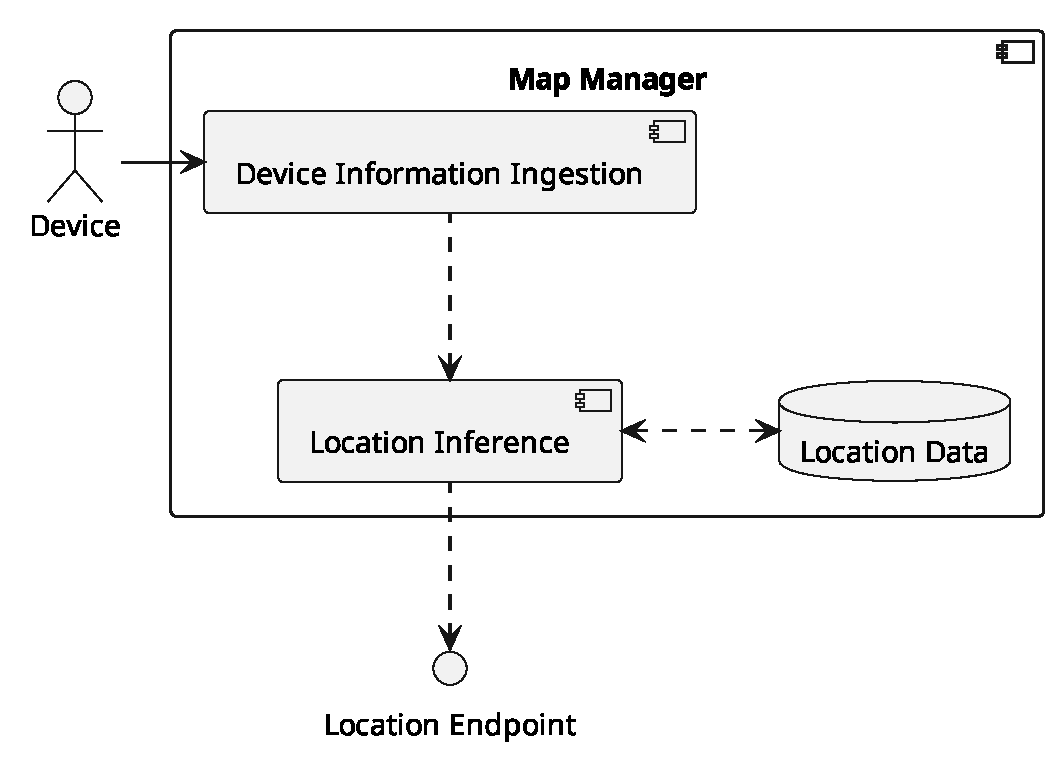
\includegraphics[width=0.7\textwidth]{img/map-manager-overview.eps}
	\caption{Component diagram showing the internal architecture of the \textit{Map Manager} component.}
	\label{fig:map-manager}
\end{figure}

Given the importance of this component and the amount of work it will have to do, attention must be paid to aspects of high availability to prevent
this component to stop working since the operation of other services depends on it.

\section{Recommendation System}

\begin{figure}[H]
	\centering
	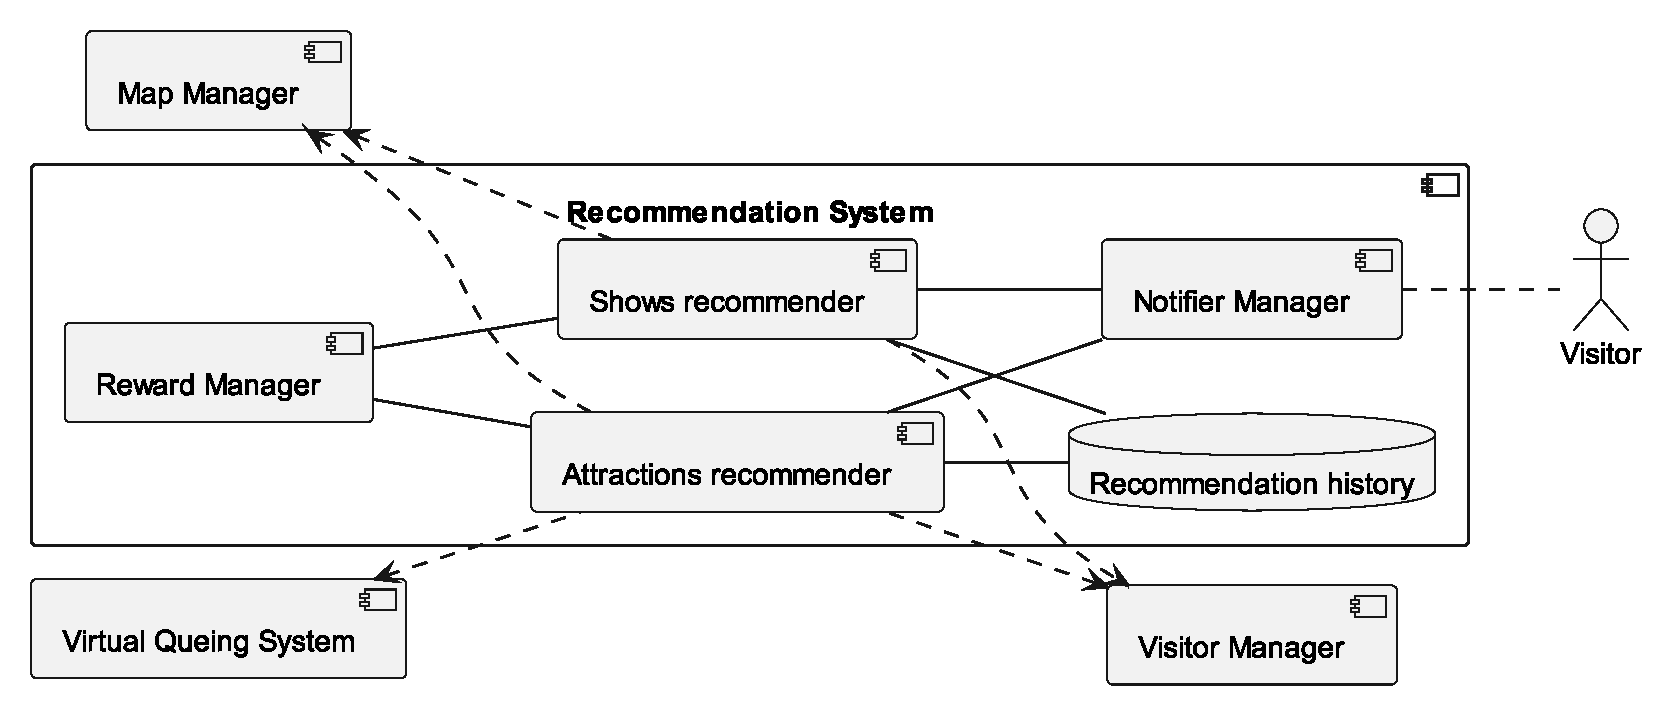
\includegraphics[width=\textwidth]{img/recommender.eps}
	\caption{Component diagram showing the internal architecture of the \textit{Recommender System}.
	}
	\label{fig:recommender-arch}
\end{figure}

The Recommendation System is a crucial component to ensure the improvement of the visitors' experience. In fact, it is responsible for collecting
data and providing tailored recommendations to the visitors and uses a Reward System to provide rewards based on the suggested actions. The
Recommendation System is composed of:
\begin{itemize}
	\item \textit{Reward Manager:} has access to all the rewards available to be given to visitors for a given recommendation. It works as previously displayed in figure~\ref{fig:reward}.
	      The visitors will receive a reward for the suggestions they take.
	\item \textit{Notification Manager:} which sends the recommendation to the visitor's wearable.
	\item \textit{Shows Recommender} and \textit{Attractions Recommender:} take visitor's information from the Visitor Manager to get their pre-compiled preferences.
	      In the former case, the subject would be shows and events they are interested in, in the latter their preferred roller coasters, shops, etc. They also get the visitors' location from the Map Manager in order to make a recommendation based on their proximity to a point of interest (\textit{situated} recommendations).
	      In addition, the Attractions Recommender uses the Virtual Queueing System data, to provide recommendations also considering the waiting time of the attractions.
	\item \textit{Recommendation History:} is responsible for storing the recommendations in order to improve the accuracy for future scenarios.
\end{itemize}

\section{Virtual Queuing System}
\begin{figure}[H]
	\centering
	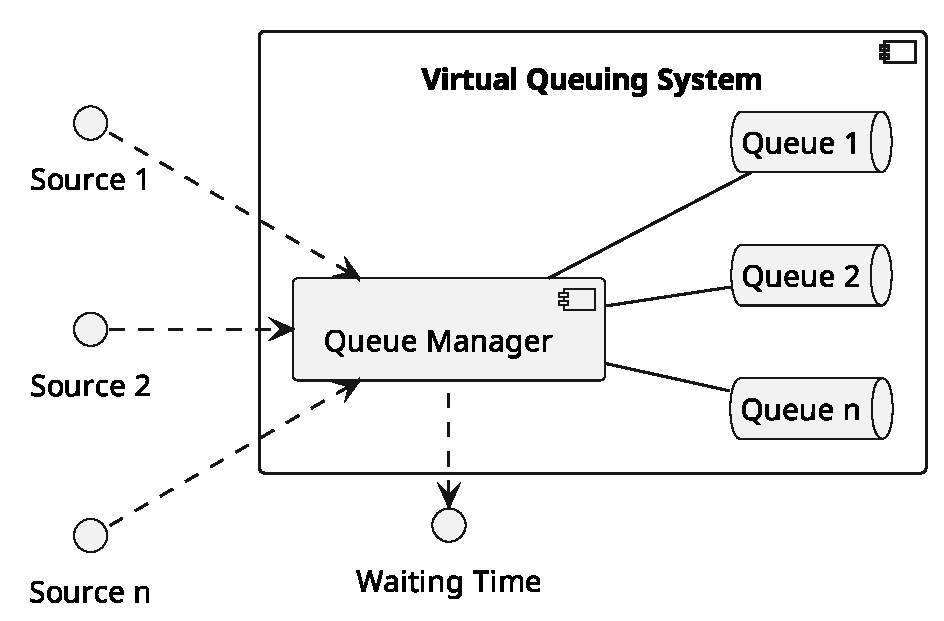
\includegraphics[width=0.7\textwidth]{img/virtual-queuing.eps}
	\caption{Component diagram showing the internal architecture of the \textit{Virtual Queueing} component.
	}
	\label{fig:virtual-queueing-arch}
\end{figure}

The Virtual Queueing System manages the waiting time of the people in the attractions queues. It could base its estimations on various sources such
as sensors (cameras, NFC, Bluetooth) or a button pressed on the visitor's wearable which communicates its presence in the queue.

The best way to implement this mechanism depends on the assumptions we could do about the context. For a Mirabilandia as a Micro City scenario, every
visitor has a wearable that allows them to enqueue themselves so we can assume that there is no need to use high or low-budget sensors: if a visitor
wants to make a ride on a roller coaster must reserve a spot in a virtual queue.

However, some sensors could be used to automatically detect corner case scenarios such as temporary roller coasters malfunctioning, bad weather etc.

\section{Planner}\label{sec:planner}

The Planner covers a main role in the overall system: the quality of experience of the user in the park depends also on it. The main goal of this
component is to satisfy as much as possible the needs and preferences expressed by visitors and at the same time ensure the best possible experience.

\begin{figure}[H]
	\centering
	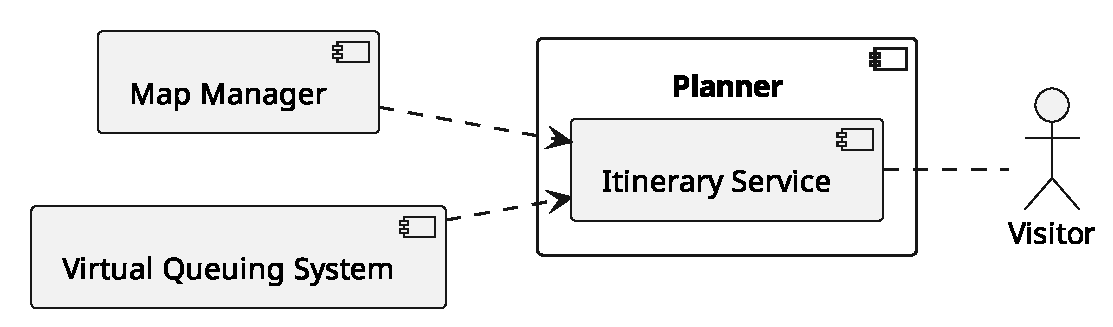
\includegraphics[width=0.7\textwidth]{img/planner.eps}
	\caption{Component diagram showing the internal architecture of the \textit{Planner} component.}
	\label{fig:planner-arch}
\end{figure}

In addition, park activities are as dynamic as park visitors are so it is easy to see that the needs of both parties may change in the process.
Therefore, it is appropriate to provide that the plans generated for visitors can change dynamically to adapt to changes in the environment. An
attraction may break down and therefore all plans that provided for the use of that ride must be adapted to the change. Again, overcrowding at an
attraction may be the reason why certain visitors' plans change to avoid excessively long queues.

From the above considerations, it is clear how the Planner needs to know in real-time: the queue status of each attraction, the preferences expressed
by each user, and the relative location within the park. Figure~\ref{fig:planner-arch} shows the dependencies that the Planner has with the rest of
the system, in particular, the information flows that the Planner needs to generate the plans are represented. The core of the \textit{Planner} is
the \textit{Itinerary Service} which collects all the information from the other components and provides the plans to each visitor.

\section{Visitors Manager}

The Visitor Manager is in charge of managing park visitor information. In particular, it is responsible for managing the visitor sign-up, the
preferences they express when accessing the park, as well as maintaining a whole range of information useful for user profiling. Moreover, the
Visitor Manager is responsible for managing the visitor's tickets, which are used to access the park and to pay for the services.

\begin{figure}[H]
	\centering
	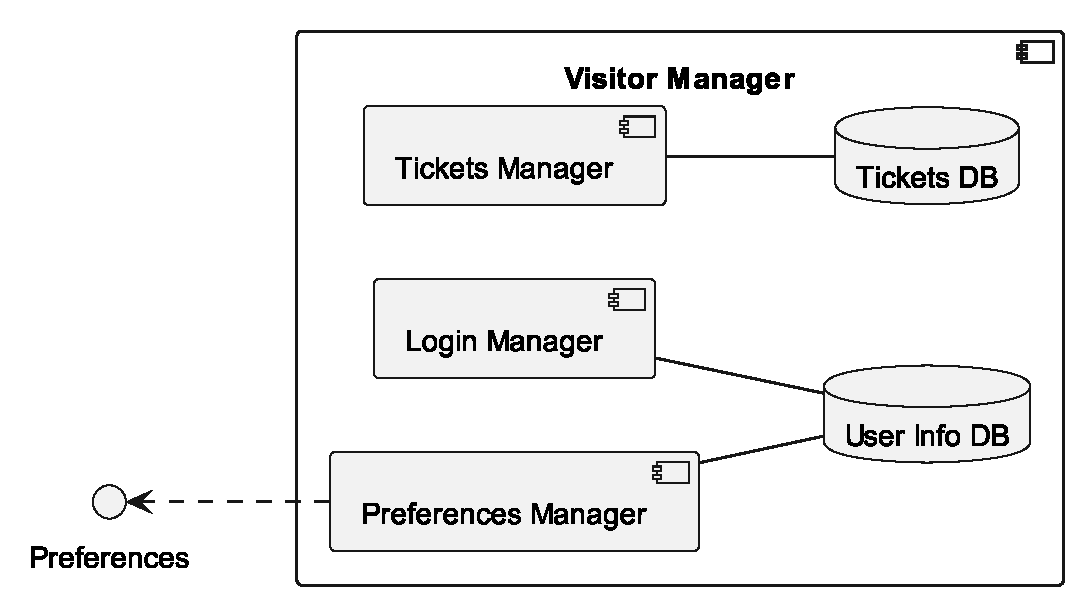
\includegraphics[width=0.7\textwidth]{img/visitor-manager.eps}
	\caption{Component diagram showing the internal architecture of the \textit{Visitor Manager} component.
	}
	\label{fig:visitor-manager-arch}
\end{figure}

The figure~\ref{fig:visitor-manager-arch} shows the internal architecture of the Visitor Manager component. The Visitor Manager is composed of three
main modules:

\begin{itemize}
	\item \textbf{Ticket Manager:} handles all the ticket-related operations like discounts, promotional offers, sales etc.
	\item \textbf{Login Manager:} handles all the login-related operations like sign-up, login, logout, password recovery etc.
	\item \textbf{Preferences Manager:} handles all the preferences related to a visitor like the preferred attractions, attractions to avoid, etc.
\end{itemize}

This component, through the data gathered from each visitor, provides the \textit{Recommender System} with the visitor's preferences.

Given the characteristics of this service and the operations it must perform, it is considered unnecessary to develop its version but rather to take
advantage of platforms already in the market that offers this kind of functionality (user management, user profiling, preference management, etc.).
For these reasons, it is not deemed necessary to examine this component further.

\section{Suitable technologies for Mirabilandia as a Micro City}
This chapter will examine in detail the technologies that are suitable for implementing the systems described above. Particularly the techniques
available for proximity marketing, crowd density estimation and people localization in indoor and outdoor environments.

\subsection{Technologies for Proximity Marketing}\label{sec:proximity-marketing-technologies}
The situated Recommendation System broadcasts notifications to devices near a certain spot. This is the same mechanism used for Proximity Marketing
techniques and seems advantageous to use the same technologies to implement such a system since there is plenty of information in the literature
regarding proximity marketing. In the following section, we will examine some of the current technologies used to implement this kind of systems.

\subsubsection{Proximity Marketing with Beacons}\label{sec:proximity-marketing-with-beacons}
Bluetooth low energy (BLE) is a Bluetooth specification designed for IoT-based applications where power consumption is a critical aspect. It is a
standard of Bluetooth that does not provide a connection functionality (pairing) but instead, transmits signals continuously. These signals can be
detected by clients that are on the lookout for that particular beacon~\cite{muddinagiri2020implementation}. Once a person with a device with
Bluetooth turned on is near the beacon, the device collects the Beacon's ID, sends it to a server that retrieves the corresponding marketing
information and returns it to the user with a message.

\subsubsection{Proximity Marketing using Wi-Fi}\label{sec:proximity-marketing-wifi}
Even though proximity-driven marketing systems have mostly been developed with the use of Bluetooth beacons~\cite{mndebele2017iot}, it is possible to
enable IoT-based proximity communication running as a service using network information, exploiting Wi-Fi. This offers better value than Bluetooth in
terms of efficiency and cost-effectiveness, as it can be used to implement IoT-based proximity solutions that run on existing infrastructure. The
detection of Wi-Fi networks already provides some data about location, namely information about proximity so proximity-based rules replace location
information, where Wi-Fi hot spots work as presence sensors~\cite{dmitry2013network}.

This paper~\cite{mndebele2017iot} for instance, presents a proximity marketing technique as a service (PMaaS). The system targets people in a
specific location and delivers messages to their mobile devices via wireless connectivity technology as long as they remain in the specified
location. Moreover, they have to be connected to a particular network segment or specific access point. To do so, the system uses network
information, i.e. the network name, and GPS parameters derived from the position of the mobile device. The marketing messages are sent by a
cloud-based platform to the eligible devices and a mobile app listens for messages applicable to the subscriber, while the subscriber is in the
relevant proximity.

\subsection{Technologies for crowd density estimation}\label{subsec:sub-ghz-wireless-sensor-network-for-crowd-density-estimation}
In our context, crowd density estimation could be advantageous to redirect visitors toward less crowded places within the park. The classic approach
to obtaining this information is to make use of an optical camera-based system but the accuracy of these systems can be rather dependent on the
lighting conditions and they tend to require the availability of a large amount of computing power. Furthermore, the use of optical cameras raises
the spectre of privacy-related issues. A WSN-based system could potentially be used to simply avoid these issues~\cite{denis2018large}. In fact, the
use of sub-GHz frequencies could be the best decision, due to their increased range and penetration capabilities through objects, walls and human
individuals~\cite{denis2018large}. Moreover, this kind of transceivers, compared to the regular Wi-Fi, have a significant lower
power-consumption~\cite{fudickar2014comparing}.

As presented in~\cite{denis2018large}, they managed to show the feasibility of using a sub-GHz wireless network to estimate the density of
large-scale crowds calculating the mean RSS-differences within a WSN between an empty and an active environment and used them as input to a
probabilistic neural network. Whereas in~\cite{fudickar2014comparing}, showed that Sub GHz transceivers achieve significant lower RSS errors and are
less influenced by obstacles attenuations. Their localisation achieved ca. 1 m more accurate median error distances than the corresponding versions
that utilise Wi-Fi transceivers. In addition, the battery runtimes are extended by 48\% when using Sub GHz transceivers instead of Wi-Fi
transceivers.

\subsection{Technologies for visitors localization}\label{sec:technologies}
Visitors localization could be useful for both proximity marketing and calculating the number of people in a queue. Indoor localization could be
helpful in our context as there are restaurants, shops and some attractions (e.g.\
Reset\footnote{\url{https://www.mirabilandia.it/en/attivita/attrazioni/reset}}) not easily reached by the outdoor localization technologies.
Moreover, the accuracy of outdoor localization technologies (e.g.\ GPS) may not be enough accurate for instance for the prize games
area\footnote{\url{https://www.mirabilandia.it/en/attivita/attrazioni/altri-giochi-e-giochi-a-premio}} where the stands are located next to each
other.

% !!! Not sure the following part fits in this section !!!
% To design and develop an effective technique for the location of visitors, the following constraints were considered:
% \begin{itemize}
% 	\item The use of a custom device is not feasible since most people reject the use of a custom device. Using each visitor's wearable would be a better choice
% 	      because they do not have the impediment of an extra device and do not need any training to use it
% 	\item The use of dedicated hardware results in an extra cost that is difficult for both the amusement park and visitors to bear.
% \end{itemize}

% Some technologies identified for these purposes will be described taking into account the constraint defined above.
% !!!!!!

\subsubsection{Wi-Fi as outdoor localization system}\label{subsec:wi-fi-as-outdoor-localization-system}

Wi-Fi is a family of wireless network protocols, which are commonly used for local area networking of devices and Internet access, allowing the
nearby digital device to exchange data by radio waves.

To date, Wi-Fi is a technology that has been pervasively adopted and made accessible to anyone because of cost, ease of installation and
configuration.

Unlike other technologies such as the global positioning system (GPS), Wi-Fi was not designed to perform device and/or person location. However, by
exploiting ad-hoc techniques it is possible to leverage this tool to perform device localization. Finally, GPS does not always perform well in any
context: in closed environments or where the GPS signal cannot reach, localization using this technology is approximate or even impractical. Another
problem with GPS is its high power consumption, which is a serious challenge to battery-based mobile devices. To tackle the problems with GPS, many
researchers have proposed a series of alternative localization schemes, including cellular-based systems~\cite{ibrahim2010cellsense}, infrared-based
systems, ultrasonic-based systems, and radio frequency (RF)-based systems~\cite{bahl2000radar, youssef2002probabilistic}.

Many researchers have proposed a variety of different schemes for outdoor localization based on mobile devices. These schemes can be divided into two
groups: range-based and range-free methods.

\begin{itemize}
	\item \textbf{Range-based}: range-based methods are mainly based on relative distance, which can be obtained through measuring methods like
	      time-of-arrival (ToA), time difference of arrival (TDoA), or propagation model generated from RSSI value.
	\item \textbf{Range-free}: one of the most widely used range-free methods is the fingerprint localization method.
	      This method can be categorized into three types:
	      visual fingerprint-based localization, motion fingerprint-based systems, and signal fingerprint-based methods.
	      In our context, the latter is the most promising.
\end{itemize}

Signal fingerprint-based localization is widely used in places where a large number of Wi-Fi infrastructures are deployed. This method commonly
consists of an offline training phase and an online fingerprint matching phase. The goal of the first phase is to form a fingerprint database that
stores the correlation between \textit{Received Signal Strength} (RSS) from various \textit{Access Points}(APs) and fixed locations. The device's
location is determined at the matching stage. In this process, we use a matching algorithm to search the fingerprint in the database which has the
minimum difference with the device that needs to be located. The associated label is our estimated location.

In terms of effect, signal fingerprint-based localization can get fine-grained results. However, as any radio environment is dynamic: unpredictable
movements of the people or large unforeseen gatherings, alterations in the radio network itself, environmental effects such as a change in humidity
levels etc.~\cite{chaudhry2013indoor} Therefore, the RF values measured for location estimation at any given point in time may significantly deviate
from those stored in the database created at the training phase~\cite{chaudhry2013indoor}. As a result, the location estimation based on a static
database may be inaccurate. Also, the training phase needs a human operator (or a human-assisted machine) to thoroughly collect the RF context and
the location from which the context was collected. To tackle these problems, as suggested in~\cite{chaudhry2013indoor}, could be useful a system that
considers the NFC technology: reference points of precisely known locations are spread in the environment, marked by NFC tags, to build the database
of fingerprints around. This could improve the training phase and allows easy adaptation to environmental changes.

\subsubsection{Bluetooth as outdoor localization system}
Bluetooth is a data transmission standard for personal wireless networks. It provides a standard way to exchange information between devices through
a short-range frequency capable of detecting devices covered by the radio signal within about ten meters by putting them in communication with each
other.

Despite being a technology conceived more than 20 years ago, it boasts massive adoption in many contexts such as medical, industrial, and in recent
years the Internet of Things (IoT). This standard was designed to achieve low power consumption, short range and a low cost of production. Over the
years, there have been several updates to the protocol, aimed at improving on the one hand the efficiency of communication by enabling higher
transmission frequencies and on the other hand improving the energy efficiency of devices.

Bluetooth was not designed to perform localization functionality. However, it is possible to exploit certain features of the protocol to make a more
or less precise estimate of a device's location. In particular, the technique most used to achieve this is based on the signal strength identified by
the RSSI (Receives Signal Strength Indicator). Other techniques, such as fingerprint-based localization can be employed to estimate position.

With the RSSI-based technique, the RSSIs of all reachable Bluetooth devices are initially acquired, and through techniques of trilateration, the
location of the device is estimated.\\ Fingerprint-based techniques estimate the location by operating in two stages: the first is the training phase
that deals with building fingerprints, which is a record that associates a location with the RSSIs of beacons reachable from that point. The second
phase involves identifying the fingerprint that least deviates from the position where the device is at a given time, and the position associated
with that fingerprint determines the estimated position. Several projects and applications rely on these two techniques to estimate the position of a
device~\cite{mcconville2021vesta, samuel2021smart}.

The proliferation of location services for various IoT applications needs to detect device locations with very high accuracies, on the order of
centimeters. With the introduction of the Bluetooth 5.1 standard, a new feature called \textit{Direction Finding} enables pinpoint localization of
Bluetooth devices. This new localization feature provides two different options for positioning a Bluetooth device, namely Angle of Arrival (AoA) and
Angle of Departure (AoD) compared to the previous version that relies only on the received signal strength indication to localize a Bluetooth device.
To be more precise, the former technique allows a receiver equipped with a multi-antenna array to identify the angular position of a transmitter
based on the phase delay of the signal received from the transmitter; the latter allows the transmitting device with multiple antennas to transmit a
radio signal that permits the receiver to determine the directional angle to the transmitter.

\section{Identified technologies to transform Mirabilandia in a Micro City}
The technologies illustrated above can be used and applied to the Mirabilandia environment. The following paragraphs have the objective to describe
how this would be possible with a fair degree of detail.
\subsection{Planner strategies and considerations}
In this section, we are not going to provide an actual technology or algorithm for making plans, but rather we want to focus on what goals an
algorithm in charge of calculating the best plan should achieve based on various factors.

As mentioned in the section~\ref{sec:planner}, we should take into account three main aspects in building the optimal plan for each visitor: the
satisfaction of the visitor's preferences, the maximization of the number of attractions visited and the minimization of the waiting time at each
attraction. The first two aspects may be similar but they are to be understood respectively as the ability to give preferences to the visitor and the
ability to maximize the number of attractions visited. The third aspect is the ability to minimize the waiting time at each attraction. The first two
aspects are related to the visitor's satisfaction, while the third aspect is related to their experience.

To evaluate the effectiveness of the plan, some metrics and indicators should be developed. Below is described a set of metrics and indicators that
could be useful in the evaluation of a plan.

\begin{itemize}
	\item \textbf{Completed Rides Indicator} (CRI): indicates the number of rides completed within one hour
	\item \textbf{Wandering Time Indicator} (WTI): indicates the quantity of time spent in the queues within one hour
	\item \textbf{User Satisfaction Indicator} (USI): indicates the number of rides completed in an hour but which were expressed as preferences by the visitor.
\end{itemize}

\begin{figure}[H]
	\centering
	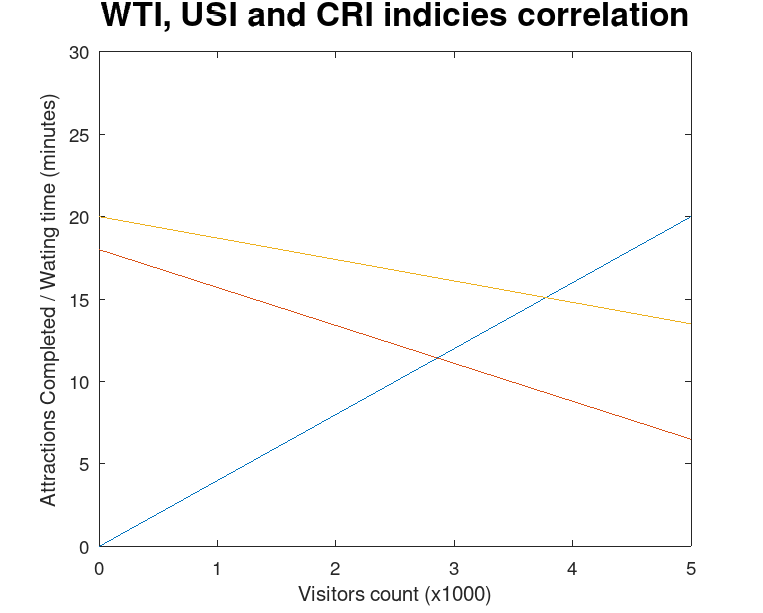
\includegraphics[width=0.8\textwidth]{img/indiciescorrelation.png}
	\caption{Correlation between the three indicators: \textit{CRI}, \textit{WTI} and \textit{USI}. This chart aims to give an empirical indication of the correlations between the three indicators. It's not based on any real data but it's a good way to understand the correlation between the three indicators.}
	\label{fig:indicies}
\end{figure}

In figure~\ref{fig:indicies}, is shown a possible correlation between the three indicators. The chart aims to provide an intuition about the trend of
the three indicators. We specify that it is not derived from any measurements nor available data, but in our opinion is a good way to get what the
indices mean.

The \textit{CRI} and \textit{USI} ad in opposition to the \textit{WTI}: if a plan is identified to provide only attractions that the user has
indicated, then the user is very likely to queue a lot and consequently increase the \textit{WTI} indicator. On the other hand, if a plan maximizes
the visitor's experience (increasing the \textit{CRI} indicator), then is quite likely that will be offered to them attractions that are not of their
interest, reducing the \textit{USI} indicator. The challenge behind the planning algorithm is to find a balance between these three indicators.

These indicators of course could be applied offline to evaluate the overall performance of the planner, but they could also be used online to adjust
in real-time the plan according to the environment changes. It is believed that a machine-learning approach could help the planning system to obtain
a better plan in real-time since it could learn from the past experiences of the visitors and adapt the plan accordingly. Moreover, due to the
complexity of the environment could not be feasible to tackle all possible scenarios, so a machine-learning approach could help to improve the plan.

\subsection{Localization techniques}
In this section, we will discuss the suitability of the localization techniques described in the previous section for Mirabilandia.

Given its size and organization, it comes naturally to think of Mirabilandia as a micro-city: streets, avenues and squares define the street network
that connects all the park's attractions and activities, just as it does for any full-scale city. The arrangement of buildings around the streets
also makes Mirabilandia a micro-city.

Given the similarities to a full-size city, we can assume with some degree of confidence that the amusement park environment is almost identical to
the city environment. Therefore, we assume that the noise and electromagnetic pollution are quite similar, and therefore all the considerations made
in the previous sections apply.

There is no definite information on the spread and coverage of Wi-Fi within the park, however, it is possible to assume that there is. Conversely, it
is by no means a given that there are Bluetooth devices that can act as beacons. In light of these considerations, we found that localization using
Wi-Fi is the most reasonable in terms of both effectiveness and cost of installation and configuration. The choice of using Wi-Fi as a technology to
support visitor tracking is based on three main considerations:

\begin{itemize}
	\item The cost of installation and configuration is relatively low since we have assumed a partially available infrastructure
	\item The spread of the technology is relatively wide, so any visitor's device support this technology.
	\item The literature about localization using Wi-Fi is relatively large, so it is feasible to use this technology.
\end{itemize}

In this scenario, Bluetooth technology has been discarded because of the low signal range and this would force the installation of many more devices
than would be needed by taking advantage of Wi-Fi; also because in outdoor environments Bluetooth provides lower guarantees in terms of signal
stability and this results in possible inaccuracies in location estimation. Finally, the introduction of the 5.1 standard is fairly new, and while it
is not a problem in terms of adoption, there are still no comprehensive studies on its effectiveness in amusement park-like environment.

Below we will illustrate a possible technique for implementing park visitor tracking by exploiting Wi-Fi as a supporting technology. The development
of this technique is based on work done by~\cite{du2018hybrid}~and~\cite{chaudhry2013indoor}.

The localization scheme consists of three main phases:

\begin{itemize}
	\item \textbf{Training phase:} in this phase, the system collects the RSSI values of the Wi-Fi APs in the park and associates them with a
	      physical position. This phase could be performed by a human operator or a human-assisted machine
	\item \textbf{Tiling phase:} in this phase the system divides the park into a grid of tiles and caches the values belonging to it
	\item \textbf{Inference phase:} in this phase the system calculates the dissimilarity between the collected patterns and the sample
	      patterns in the database built before. The location of the fingerprint with the minimum difference will be selected as an estimation for the
	      location of the device.
\end{itemize}

The \textit{training phase} is the most important and challenging phase of the scheme. It is the phase in which the system collects the RSSI values
of the Wi-Fi APs in the park and associates them with a physical position. The accuracy of this phase is crucial: a wrong position in a fingerprint
could result in inaccurate location estimation. The collection of the fingerprint database could be done in several ways: by a human operator, which
walking around the park collects the RSSI values of the Wi-Fi APs and associates them with a physical position, creating a fingerprint record.
Alternatively, a fleet of robots (like drones) could be used to collect the RSSI values and associate them with a physical position. This scenario is
ambitious but could be faster and less error-prone than the human ones.

The \textit{tile phase} consists of a series of optimizations exploited by the \textit{inference phase} to reduce the inference time. The map is
divided into regions, each containing fingerprints of the locations contained in it. In this way, it is not required to use the entire fingerprint
database, but only the region (or regions) of interest. Finally, each tile can be cached for additional performance improvements during the inference
phase. Determining which tile should be used for the inference step is not an easy task. Choosing the wrong tile may result in an incorrect position
estimate. At the same time, it is particularly inefficient to estimate the position by leveraging the entire fingerprint database. For this reason, a
sensor-assisted matching method can restrict the matching operation in a small space through sensor information including direction and travel
distance. The current location can be calculated from an initial location, which can be taken from the GPS, for example. The distance and direction
can be estimated using the dead reckoning~\footnote{\url{https://en.wikipedia.org/wiki/Dead_reckoning}} method with built-in inertial sensors like
accelerometer, gyroscope, and compass. Given the longitude and latitude of the start point, the distance and bearing from the start point, and the
destination point can be calculated using the Haversine formula~\footnote{\url{https://en.wikipedia.org/wiki/Haversine_formula}}. In this way, a
subset of the local fingerprint database cache can be obtained.

The \textit{inference phase} is the most important phase of the scheme. It is the phase in which the system calculates the position of the device.
Let's denote by $f = {r_1, r_2, \ldots, r_n}$ a \textit{fingerprint} record where $r_i$ represents the RSS value of captured AP and $n$ the number of
APs in the fingerprint record. Let's calculate the dissimilarity between two fingerprints based on the RSSI difference. Denote with $\sigma_i = | r_i
	- r^{'}_{i}|$ the difference of fingerprints $f^{'}$ and $f$ at each $A_i$ where $A_i \in A$ where $A$ is the fingerprint database. Since two
fingerprints may contain a different set of APs, the access point $A_i$ may appear in $f$ but does not appear in $f^{'}$. For this situation, we
assume the signal strength is weak and let the missing value equal to $-100$. The dissimilarity between $f$ and $f^{'}$ is calculated via the
following formula:

\begin{equation}
	\eta(f, f^{'}) = \sqrt{\sum_{i=0}^{p} \sigma_i^{2}}
	\label{eq:dissimilarity}
\end{equation}

where $p = | A \cup A^{'} |$

The location is calculated via the sample with minimum dissimilarity by comparing all samples stored in the fingerprint database $F$ with the query
fingerprint $f$.

\begin{equation}
	f^{*} = \arg \min_{f_i \in F} \ \eta(f, f_i)
	\label{eq:min-dissimilarity}
\end{equation}

$L(f^{*})$ is the corresponding location of $f^{*}$ which represents the estimated place.

As can be seen from formula~\ref{eq:min-dissimilarity}, the iteration over all fingerprints cannot scale at all: the time needed to iterate all the
fingerprints are proportional to the number of them. In large maps, the number of fingerprints could become very huge degrading the inference time.
It is in this situation that tiling improves performance due to dimension reduction; this reduction is determined by the $k$ factor, where $k$ is the
number of tiles of the map.

\begin{figure}[H]
	\centering
	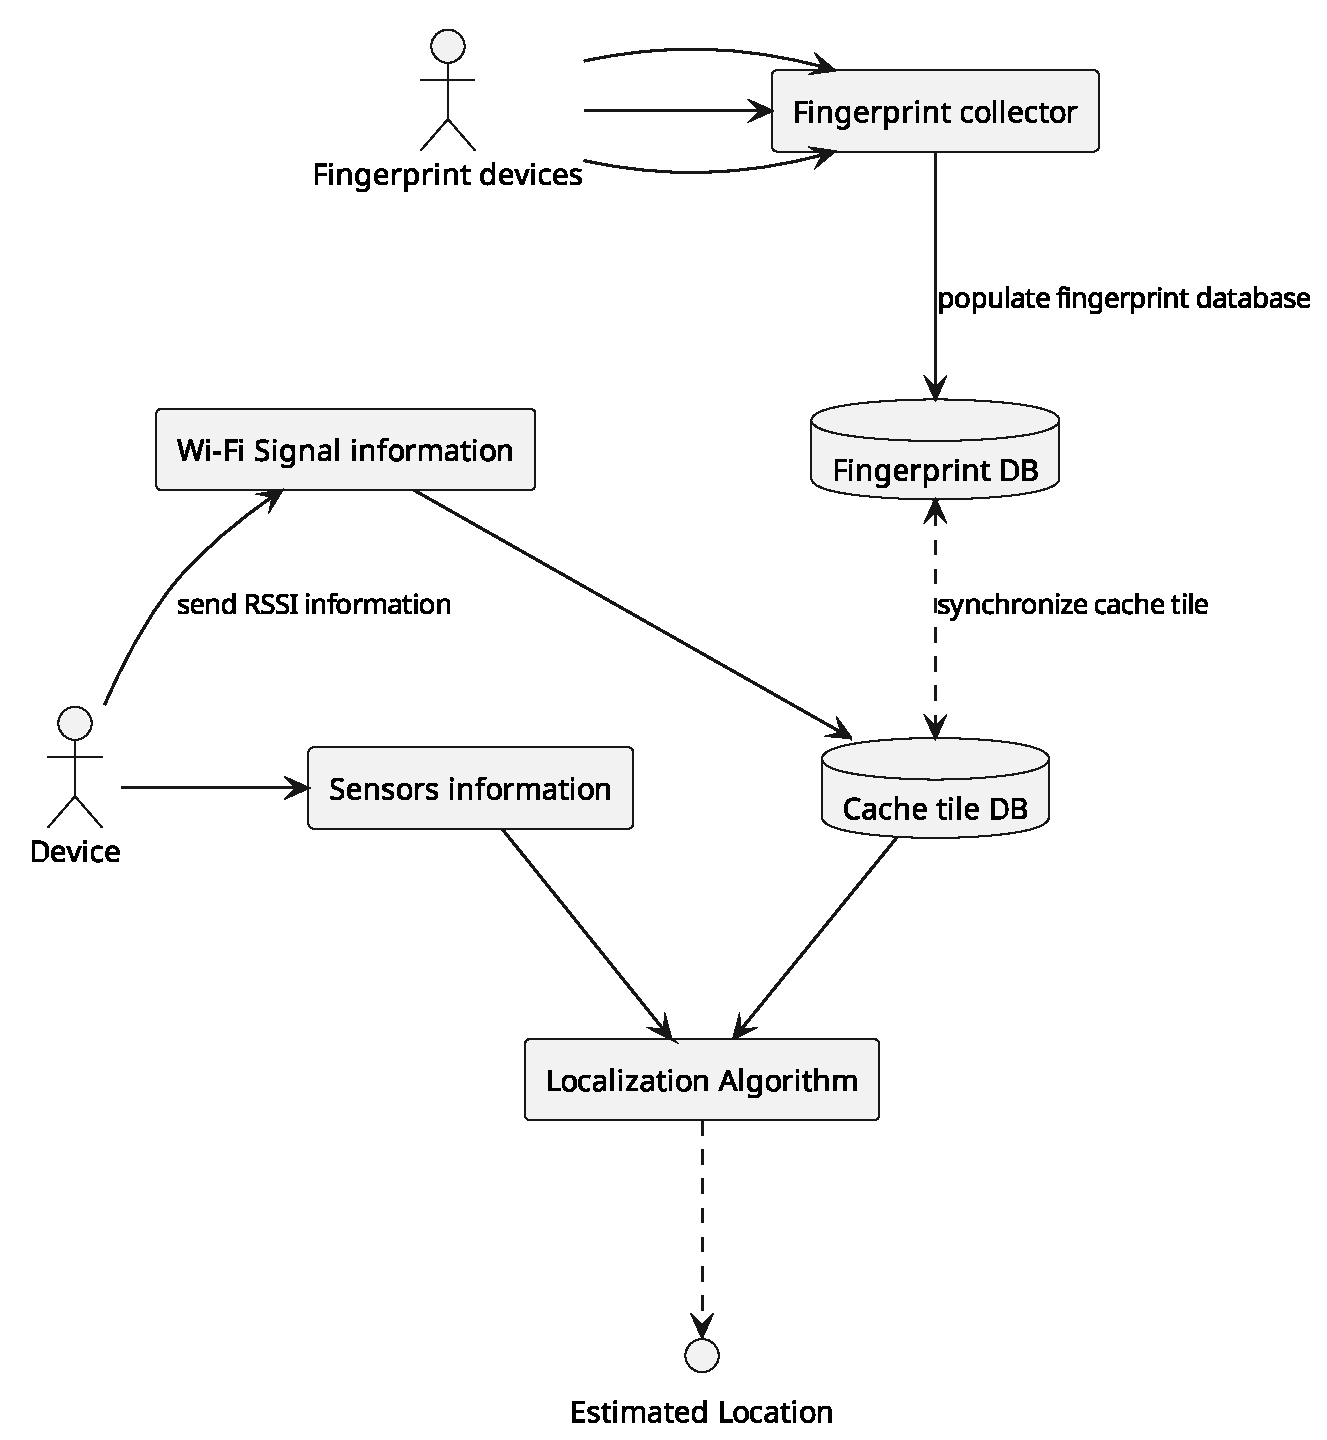
\includegraphics[width=0.7\textwidth]{img/fingerprint-schema.eps}
	\caption{Main steps in the proposed schema for Wi-Fi fingerprint-based localization technique.}
	\label{fig:fingerprint-schema}
\end{figure}

In figure~\ref{fig:fingerprint-schema} are summarized the steps for the localization based on Wi-Fi.

The adoption of this technique leads to several advantages:
\begin{itemize}
	\item The accuracy of the localization is improved compared with the GPS one~\cite{du2018hybrid}
	\item The power consumption needed to implement this system is sensible lower than the GPS~\cite{du2018hybrid}
	\item The flexibility of this technique enables the computation of the location either on the device or on the server.
\end{itemize}

We believe that Wi-Fi-based calculation of visitor location within the amusement park is a promising solution in terms of both effectiveness (more
accurate location and lower consumption) and costs instead of using a traditional system like GPS.

\subsection{Situated Recommendation system}\label{sec:situated-recommendation-sys}
To implement the situated Recommendation system in Mirabilandia we could assume that the technology for detecting the presence of a visitor in a
certain spot could be abstracted.

In fact, could be sufficient to associate the location of the visitor with an ID and the ID with an action. Then the system sends a recommendation
for the user based on the action, the position and the visitor's information. generates This way, the ``situated'' part of the system can be
implemented in a very simple way: every location of interest is previously set and every time a visitor is near, sends to the visitor's wearable its
id. Then, the wearable sends to the recommendation system the visitor's info and the collected id, checks the correspondence of the id with an
action, decides if the visitor is feasible to get the corresponding recommendation and, if so, sends the recommendation to the visitor. The
Recommendation System will implement the usual Machine Learning algorithms to take the decision of sending a recommendation.

The sequence diagram of the process is shown in Figure~\ref{fig:situated-recommendation}.

\begin{figure}[H]
	\centering
	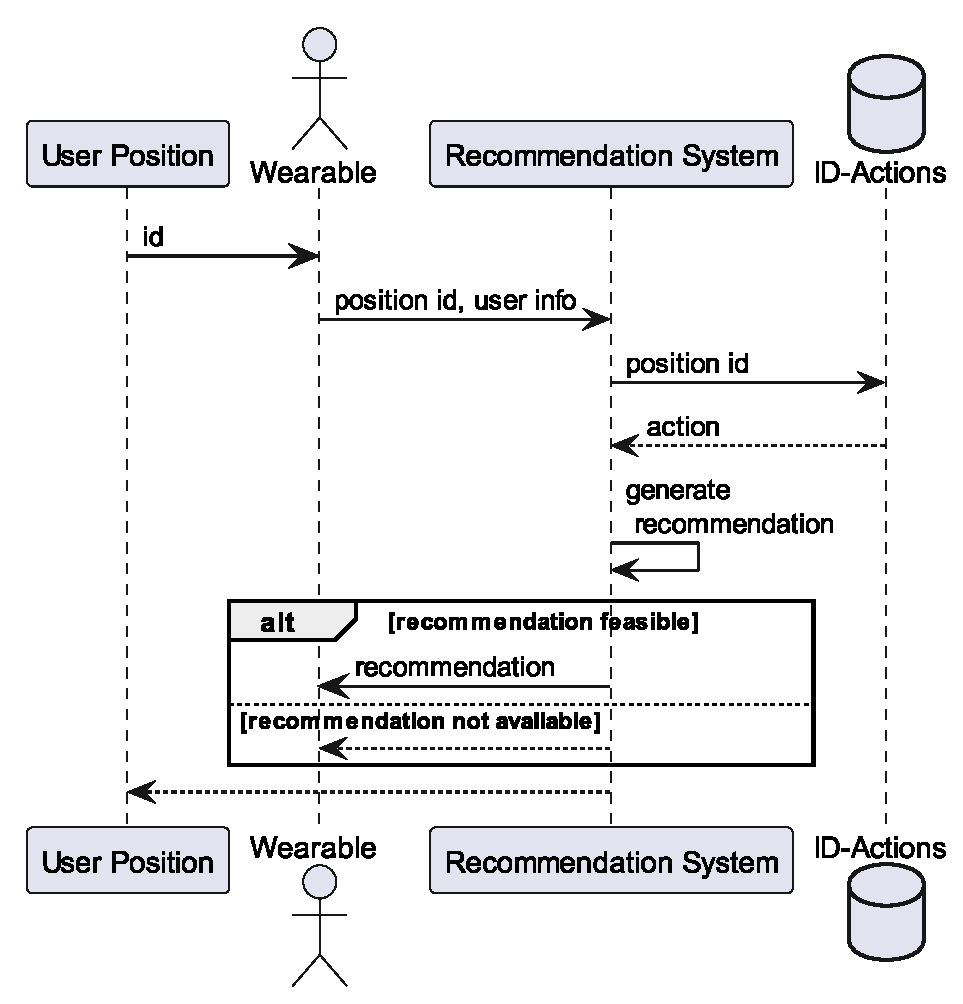
\includegraphics[width=0.7\textwidth]{img/seq_diag_situated.eps}
	\caption{Situated Recommendation System activity diagram.}
	\label{fig:situated-recommendation}
\end{figure}

\section{Deployment strategy for a real case scenario}
In this section, we will examine a possible deployment strategy for the proposed system. In particular, we will take into account all the pros and
cons of a full cloud solution, a full fog solution, and a hybrid solution.

\subsection{Fog computing}
Traditional cloud-based IoT systems are challenged by the large scale, heterogeneity, and high latency witnessed in some cloud ecosystems. Fog
computing is a possible solution as it's a distributed computing paradigm that extends cloud computing to the edge of the network: it allows the
decentralization of applications, management, data analytics, etc. into the network itself.

This model enables ubiquitous access to a shared continuum of scalable computing resources. The deployment of distributed, latency-aware applications
and services is facilitated and consists of fog nodes (physical or virtual), residing between smart end devices and centralized (cloud) services. The
fog nodes are context-aware and support a common data management and communication system. They can be organized in clusters - either vertically (to
support isolation), horizontally (to support federation), or relative to fog nodes' latency distance to the smart end devices. Fog computing
minimizes the request-response time from/to supported applications, and provides, for the end-devices, local computing resources and, when needed,
network connectivity to centralized services~\cite{iorga2018fog}.

This is an interesting model for some components of our use case.

\subsection{Fog computing vs Cloud computing}
First, it's important to understand that cloud and fog computing are different, noninterchangeable technologies that cannot replace one another. Fog
computing is used to process time-sensitive data, while cloud computing is used to process data that is not time-driven. While cloud computing is
designed to provide high availability and on-demand scaling, the latency introduced by the communication could increase a lot the response time. Fog
computing is designed to reduce latency by processing data locally. The main advantage of fog computing is the reduction of latency, but it has some
drawbacks. The main one is the lack of scalability. Fog computing is not designed to scale, so it's not possible to add more nodes to increase
processing power. Another drawback is the high cost of the infrastructure.

Thus, we can conclude that the cloud has the advantages of providing high computing power and scaling on demand; on the other hand, it has as its
main disadvantage the high delay in communication between devices and the cloud itself. On the other hand, the fog has the disadvantage of having
limited computational resources and higher utilization costs but has the advantage of having very fast communication times with devices.

\subsection{Hybrid architecture: cloud, fog and edge}\label{sec:hybrid-arch}
The advantages of one approach and the other do not by themselves justify the choice of one or the other. Rather, we believe that the adoption of all
the technologies leads to a concrete advantage in the realization of Mirabilandia as a Micro City.

We then go on to analyze the requirements of each system component described in section~\ref{sec:mira-microcity}, and for each one, we will identify
whether it is best implemented in a cloud, fog or edge context.

\subsubsection{Mirabilanda Micro City deployment architecture}
In figure~\ref{fig:deployment} is shown a possible deployment strategy for the Mirabilandia Micro City. The architecture is based on the hybrid
architecture described in section~\ref{sec:hybrid-arch}.

\begin{figure}[H]
	\centering
	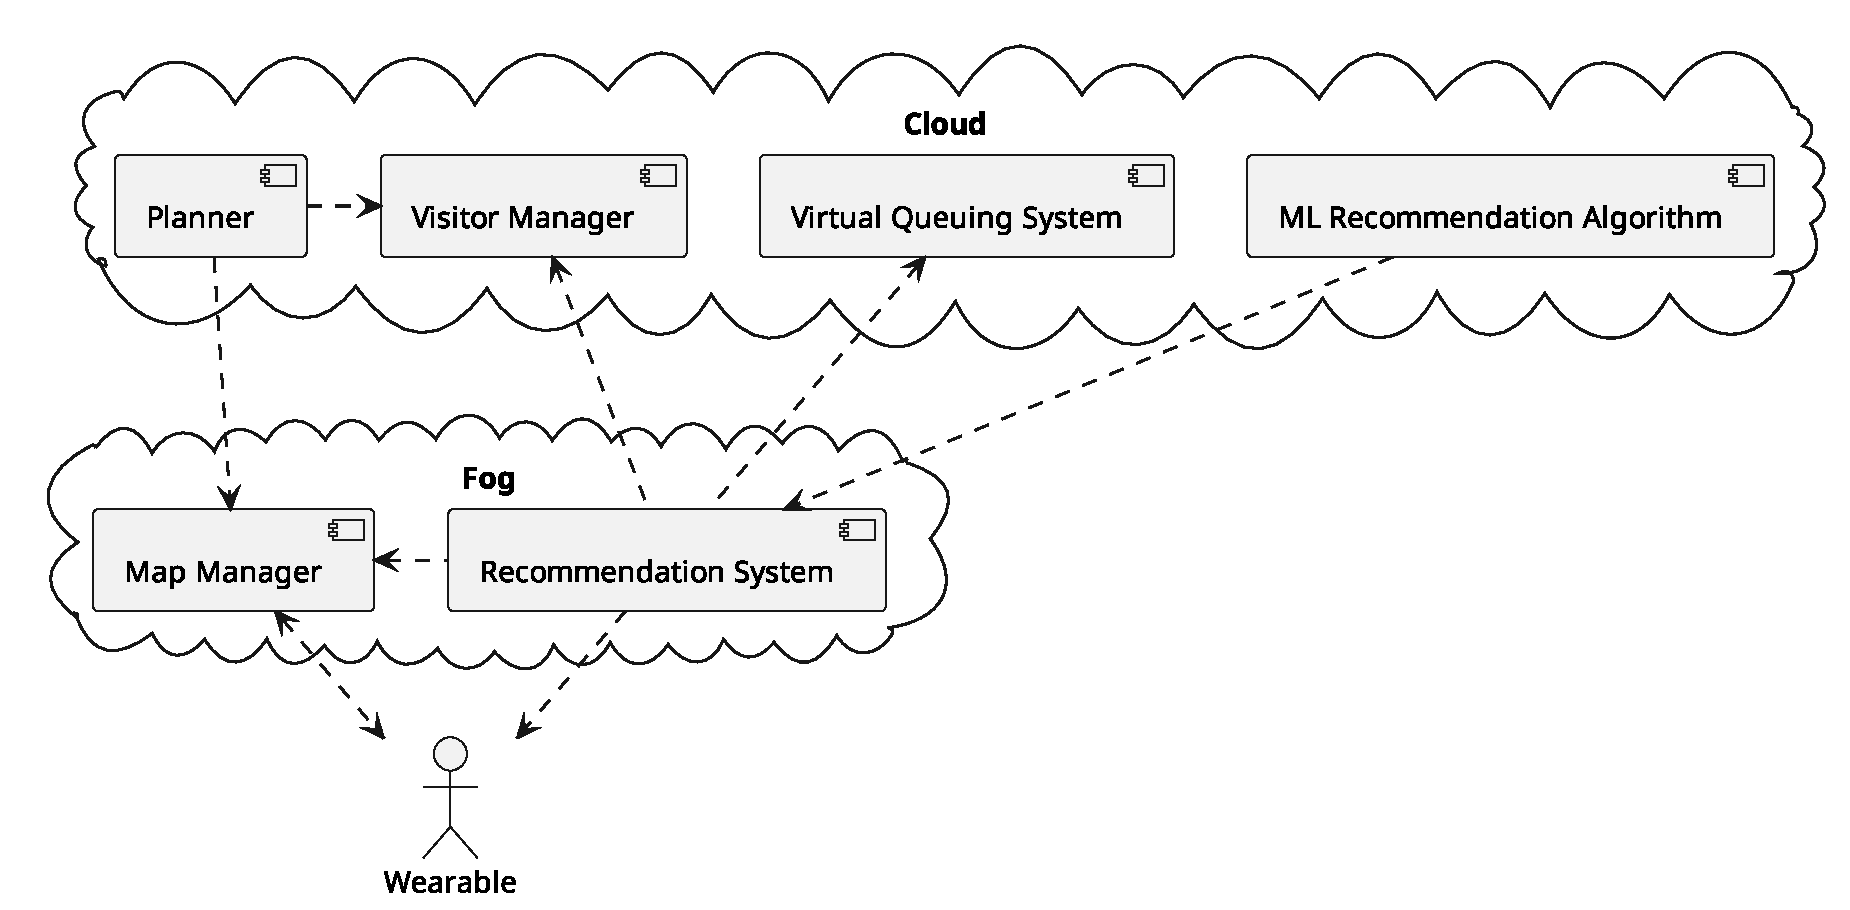
\includegraphics[width=\textwidth]{img/deployment.eps}
	\caption{Component diagram showing a possible deployment strategy for the Mirabilandia Micro City.}
	\label{fig:deployment}
\end{figure}

In the following sections, we will describe in detail all the deployment strategies for each component of the Mirabilandia Micro City.

\subsubsection{Recommendation System deployment strategy}
As we previously said in other sections, our situated Recommendation System is similar to a Proximity Marketing system. Thus, the deployment strategy
could use some state-of-the-art technologies that can be found in the literature regarding this topic. Mirabilandia has a large number of visitors
every day and current technology infrastructures and architectures need to be designed to process in real-time the great amount of information data
that is being made available from such several devices with a so high concentration. Given that, our solution will provide the system with a
three-layered structure: the edge layer, the fog layer and the cloud layer:
\begin{itemize}
	\item The edge layer will be composed of the devices that will contain the visitors' information, as well as the id of their position - as per
	      section~\ref{sec:situated-recommendation-sys}. These devices will send that information to the fog layer.
	\item The fog layer provides real-time computing and storage resources to the edge elements. The \textit{Recommendation System} is placed here since a
	      recommendation should occur as quickly as possible since the visitor's position could change within seconds.
	\item The cloud layer provides scalable computing power for machine learning algorithms to aggregate useful information for the \textit{Recommendation
		      System} components in the fog layer.
\end{itemize}

\subsubsection{Virtual Queueing System deployment strategy}
Even though the Virtual Queueing System should be fairly fast in calculating the waiting time - since it should be updated every time a visitor enter
or leaves the queue or an external event occurs - we believe that the cloud is the best solution for this system. In fact, as long as the visitor is
notified of the waiting time, it doesn't need to be updated in real-time. The Virtual Queueing System could use machine learning algorithms to better
do its calculations considering the guest's flow, bad weather, ride downtime etc. and therefore it needs a lot of computing power. The cloud is the
best solution for these operations and it allows to scale of the resources implied depending on the number of visitors.

\subsubsection{Visitor Manager deployment strategy}
Concerning the \textit{Visitor Manager} component, this has no particular constraints either in terms of computational complexity or latency in
communications; dealing mainly with managing user master data and their preferences in addition to being in charge of ticket sales, this component
can exist in a cloud context or an external CRM can be leveraged.

\subsubsection{Planner deployment strategy}
The \textit{Planner} is responsible for managing the plans for each park visitor. This task requires fairly high computational capabilities since the
plan can evolve. Although itinerary management is a relevant aspect, the speed of plan generation is not considered of primary importance. Even if
the updated plan is propagated to visitors within a few seconds or a few tens of seconds, it is not believed to infect the overall visitor
experience. Given these requirements, it is believed that a cloud solution can adhere well to the needs of this component. The choice of the cloud is
further strengthened by the fact that the computational requirements can vary quite a bit over time: there may be times of the year when the
attendance of people at the amusement park is rather limited, so the plans to be calculated turn out to be fewer in number and therefore less
computational capacity is required. Conversely, on the other hand, at peak times visitor turnout requires significantly increased computational
capacity to meet the demands. The dynamism with which resources can be allocated or de-allocated is something that the cloud natively handles, thus
representing the optimal solution for implementing such a service.

\subsubsection{Map Manager deployment strategy}
The \textit{Map Manager} is responsible for maintaining information on the location of each visitor within the park. It is the component that has the
most interaction with visitor devices and the one that requires a near-real-time operation. This component requires component-device communication to
be as fast as possible to calculate the corresponding location. In this context, the computational complexity required for position computation is
not very high, but low latency in communications is required. For this reason, a fog solution would be ideal to implement such a system. To further
reduce the latency in communication, it is possible to think of a hybrid scenario: initially, it is the device that, using the same algorithm,
estimates its position within the park and directly sends the position information to the service. In this way, the \textit{Map Manager} acts as an
aggregator of information that it then makes available to the other services. If the device fails to compute the position promptly or due to other
factors it is deemed that the computation should be done offline, then the device reverts to operating as described above, i.e., it sends only the
information that is useful for making the position computation, which will be done by the \textit{Map Manager}. In this way, one can
opportunistically determine where it is best to perform the computation of the position estimate.


\chapter{Conclusions}\label{chap:conclusions}
In this paper we have formalized the concept of Micro City, defining its aspects and characteristics that determine its distinctiveness. 

We identified the amusement park as a possible scenario in which this concept could be applied and analyzed the case-study-specific characteristics.

At a later time, we conducted research about amusement parks in general and what are the technologies they currently use to improve the visitors' experience.
Then, we chose Mirabilandia as a real-world amusement park case study, conducting an analysis of the current technological status made available to the park and then focusing on what cutting-edge technologies could implement our Micro City concept.
In particular, the state of the art about situated recommendation techniques and visitor location exploiting Wi-Fi networks to increase location accuracy were studied. 

Finally, some considerations were made about possible choices for deploying a working system.

This project gave us the opportunity to engage in identifying, developing and partly formalizing an entirely new model. 

It allowed us to study the literature on areas we had never explored before and then adapt the notions learned to our Micro City context.

It was challenging to adapt the theorized concepts into a real-world case study, but we feel satisfied with the results obtained despite the short time available.


\nocite{*}
\newpage
\printbibliography[heading=bibintoc]

\end{document}